% Options for packages loaded elsewhere
\PassOptionsToPackage{unicode}{hyperref}
\PassOptionsToPackage{hyphens}{url}
\PassOptionsToPackage{dvipsnames,svgnames,x11names}{xcolor}
%
\documentclass[
  12pt,
  letterpaper,
]{book}

\usepackage{amsmath,amssymb}
\usepackage{iftex}
\ifPDFTeX
  \usepackage[T1]{fontenc}
  \usepackage[utf8]{inputenc}
  \usepackage{textcomp} % provide euro and other symbols
\else % if luatex or xetex
  \usepackage{unicode-math}
  \defaultfontfeatures{Scale=MatchLowercase}
  \defaultfontfeatures[\rmfamily]{Ligatures=TeX,Scale=1}
\fi
\usepackage{lmodern}
\ifPDFTeX\else  
    % xetex/luatex font selection
\fi
% Use upquote if available, for straight quotes in verbatim environments
\IfFileExists{upquote.sty}{\usepackage{upquote}}{}
\IfFileExists{microtype.sty}{% use microtype if available
  \usepackage[]{microtype}
  \UseMicrotypeSet[protrusion]{basicmath} % disable protrusion for tt fonts
}{}
\makeatletter
\@ifundefined{KOMAClassName}{% if non-KOMA class
  \IfFileExists{parskip.sty}{%
    \usepackage{parskip}
  }{% else
    \setlength{\parindent}{0pt}
    \setlength{\parskip}{6pt plus 2pt minus 1pt}}
}{% if KOMA class
  \KOMAoptions{parskip=half}}
\makeatother
\usepackage{xcolor}
\usepackage[margin=1in]{geometry}
\setlength{\emergencystretch}{3em} % prevent overfull lines
\setcounter{secnumdepth}{5}
% Make \paragraph and \subparagraph free-standing
\makeatletter
\ifx\paragraph\undefined\else
  \let\oldparagraph\paragraph
  \renewcommand{\paragraph}{
    \@ifstar
      \xxxParagraphStar
      \xxxParagraphNoStar
  }
  \newcommand{\xxxParagraphStar}[1]{\oldparagraph*{#1}\mbox{}}
  \newcommand{\xxxParagraphNoStar}[1]{\oldparagraph{#1}\mbox{}}
\fi
\ifx\subparagraph\undefined\else
  \let\oldsubparagraph\subparagraph
  \renewcommand{\subparagraph}{
    \@ifstar
      \xxxSubParagraphStar
      \xxxSubParagraphNoStar
  }
  \newcommand{\xxxSubParagraphStar}[1]{\oldsubparagraph*{#1}\mbox{}}
  \newcommand{\xxxSubParagraphNoStar}[1]{\oldsubparagraph{#1}\mbox{}}
\fi
\makeatother

\usepackage{color}
\usepackage{fancyvrb}
\newcommand{\VerbBar}{|}
\newcommand{\VERB}{\Verb[commandchars=\\\{\}]}
\DefineVerbatimEnvironment{Highlighting}{Verbatim}{commandchars=\\\{\}}
% Add ',fontsize=\small' for more characters per line
\usepackage{framed}
\definecolor{shadecolor}{RGB}{241,243,245}
\newenvironment{Shaded}{\begin{snugshade}}{\end{snugshade}}
\newcommand{\AlertTok}[1]{\textcolor[rgb]{0.68,0.00,0.00}{#1}}
\newcommand{\AnnotationTok}[1]{\textcolor[rgb]{0.37,0.37,0.37}{#1}}
\newcommand{\AttributeTok}[1]{\textcolor[rgb]{0.40,0.45,0.13}{#1}}
\newcommand{\BaseNTok}[1]{\textcolor[rgb]{0.68,0.00,0.00}{#1}}
\newcommand{\BuiltInTok}[1]{\textcolor[rgb]{0.00,0.23,0.31}{#1}}
\newcommand{\CharTok}[1]{\textcolor[rgb]{0.13,0.47,0.30}{#1}}
\newcommand{\CommentTok}[1]{\textcolor[rgb]{0.37,0.37,0.37}{#1}}
\newcommand{\CommentVarTok}[1]{\textcolor[rgb]{0.37,0.37,0.37}{\textit{#1}}}
\newcommand{\ConstantTok}[1]{\textcolor[rgb]{0.56,0.35,0.01}{#1}}
\newcommand{\ControlFlowTok}[1]{\textcolor[rgb]{0.00,0.23,0.31}{\textbf{#1}}}
\newcommand{\DataTypeTok}[1]{\textcolor[rgb]{0.68,0.00,0.00}{#1}}
\newcommand{\DecValTok}[1]{\textcolor[rgb]{0.68,0.00,0.00}{#1}}
\newcommand{\DocumentationTok}[1]{\textcolor[rgb]{0.37,0.37,0.37}{\textit{#1}}}
\newcommand{\ErrorTok}[1]{\textcolor[rgb]{0.68,0.00,0.00}{#1}}
\newcommand{\ExtensionTok}[1]{\textcolor[rgb]{0.00,0.23,0.31}{#1}}
\newcommand{\FloatTok}[1]{\textcolor[rgb]{0.68,0.00,0.00}{#1}}
\newcommand{\FunctionTok}[1]{\textcolor[rgb]{0.28,0.35,0.67}{#1}}
\newcommand{\ImportTok}[1]{\textcolor[rgb]{0.00,0.46,0.62}{#1}}
\newcommand{\InformationTok}[1]{\textcolor[rgb]{0.37,0.37,0.37}{#1}}
\newcommand{\KeywordTok}[1]{\textcolor[rgb]{0.00,0.23,0.31}{\textbf{#1}}}
\newcommand{\NormalTok}[1]{\textcolor[rgb]{0.00,0.23,0.31}{#1}}
\newcommand{\OperatorTok}[1]{\textcolor[rgb]{0.37,0.37,0.37}{#1}}
\newcommand{\OtherTok}[1]{\textcolor[rgb]{0.00,0.23,0.31}{#1}}
\newcommand{\PreprocessorTok}[1]{\textcolor[rgb]{0.68,0.00,0.00}{#1}}
\newcommand{\RegionMarkerTok}[1]{\textcolor[rgb]{0.00,0.23,0.31}{#1}}
\newcommand{\SpecialCharTok}[1]{\textcolor[rgb]{0.37,0.37,0.37}{#1}}
\newcommand{\SpecialStringTok}[1]{\textcolor[rgb]{0.13,0.47,0.30}{#1}}
\newcommand{\StringTok}[1]{\textcolor[rgb]{0.13,0.47,0.30}{#1}}
\newcommand{\VariableTok}[1]{\textcolor[rgb]{0.07,0.07,0.07}{#1}}
\newcommand{\VerbatimStringTok}[1]{\textcolor[rgb]{0.13,0.47,0.30}{#1}}
\newcommand{\WarningTok}[1]{\textcolor[rgb]{0.37,0.37,0.37}{\textit{#1}}}

\providecommand{\tightlist}{%
  \setlength{\itemsep}{0pt}\setlength{\parskip}{0pt}}\usepackage{longtable,booktabs,array}
\usepackage{calc} % for calculating minipage widths
% Correct order of tables after \paragraph or \subparagraph
\usepackage{etoolbox}
\makeatletter
\patchcmd\longtable{\par}{\if@noskipsec\mbox{}\fi\par}{}{}
\makeatother
% Allow footnotes in longtable head/foot
\IfFileExists{footnotehyper.sty}{\usepackage{footnotehyper}}{\usepackage{footnote}}
\makesavenoteenv{longtable}
\usepackage{graphicx}
\makeatletter
\def\maxwidth{\ifdim\Gin@nat@width>\linewidth\linewidth\else\Gin@nat@width\fi}
\def\maxheight{\ifdim\Gin@nat@height>\textheight\textheight\else\Gin@nat@height\fi}
\makeatother
% Scale images if necessary, so that they will not overflow the page
% margins by default, and it is still possible to overwrite the defaults
% using explicit options in \includegraphics[width, height, ...]{}
\setkeys{Gin}{width=\maxwidth,height=\maxheight,keepaspectratio}
% Set default figure placement to htbp
\makeatletter
\def\fps@figure{htbp}
\makeatother

% header.tex
\usepackage{xcolor}        % Para colores
\usepackage{polyglossia}   % Soporte de idiomas con XeLaTeX
\setdefaultlanguage{spanish}

% Definición de colores personalizados
\definecolor{fecundidad}{HTML}{FFC125}      % Amarillo
\definecolor{supervivencia}{HTML}{36648B}   % Azul
\definecolor{crecimiento}{HTML}{548B54}     % Verde
\definecolor{retroceso}{HTML}{7A378B}       % Violeta
\definecolor{permanencia}{HTML}{26466A}     % Azul oscuro
\usepackage{booktabs}
\usepackage{caption}
\usepackage{longtable}
\usepackage{colortbl}
\usepackage{array}
\usepackage{anyfontsize}
\usepackage{multirow}
\makeatletter
\@ifpackageloaded{caption}{}{\usepackage{caption}}
\AtBeginDocument{%
\ifdefined\contentsname
  \renewcommand*\contentsname{Table of contents}
\else
  \newcommand\contentsname{Table of contents}
\fi
\ifdefined\listfigurename
  \renewcommand*\listfigurename{List of Figures}
\else
  \newcommand\listfigurename{List of Figures}
\fi
\ifdefined\listtablename
  \renewcommand*\listtablename{List of Tables}
\else
  \newcommand\listtablename{List of Tables}
\fi
\ifdefined\figurename
  \renewcommand*\figurename{Figure}
\else
  \newcommand\figurename{Figure}
\fi
\ifdefined\tablename
  \renewcommand*\tablename{Table}
\else
  \newcommand\tablename{Table}
\fi
}
\@ifpackageloaded{float}{}{\usepackage{float}}
\floatstyle{ruled}
\@ifundefined{c@chapter}{\newfloat{codelisting}{h}{lop}}{\newfloat{codelisting}{h}{lop}[chapter]}
\floatname{codelisting}{Listing}
\newcommand*\listoflistings{\listof{codelisting}{List of Listings}}
\makeatother
\makeatletter
\makeatother
\makeatletter
\@ifpackageloaded{caption}{}{\usepackage{caption}}
\@ifpackageloaded{subcaption}{}{\usepackage{subcaption}}
\makeatother

\ifLuaTeX
  \usepackage{selnolig}  % disable illegal ligatures
\fi
\usepackage{bookmark}

\IfFileExists{xurl.sty}{\usepackage{xurl}}{} % add URL line breaks if available
\urlstyle{same} % disable monospaced font for URLs
\hypersetup{
  colorlinks=true,
  linkcolor={Maroon},
  filecolor={Maroon},
  citecolor={Blue},
  urlcolor={Blue},
  pdfcreator={LaTeX via pandoc}}


\author{}
\date{}

\begin{document}
\frontmatter

\renewcommand*\contentsname{Table of contents}
{
\hypersetup{linkcolor=}
\setcounter{tocdepth}{2}
\tableofcontents
}

\mainmatter
\chapter{Largo y Expectativa de Vida}\label{largo-y-expectativa-de-vida}

\begin{Shaded}
\begin{Highlighting}[]
\FunctionTok{library}\NormalTok{(Rcompadre) }\CommentTok{\# Paquete para trabajar con la base de datos de COMPADRE y COMADRE}
\FunctionTok{library}\NormalTok{(tidyverse) }\CommentTok{\# Paquete para activar multiples paquetes}
\FunctionTok{library}\NormalTok{(Rage) }\CommentTok{\# Paquete para calcular métricas demográficas a partir de matrices de proyección}
\FunctionTok{library}\NormalTok{(gt) }\CommentTok{\# Paquete para crear tablas bonitas}
\end{Highlighting}
\end{Shaded}

\begin{Shaded}
\begin{Highlighting}[]
\NormalTok{compadre }\OtherTok{\textless{}{-}} \FunctionTok{cdb\_fetch}\NormalTok{(}\StringTok{"compadre"}\NormalTok{) }\CommentTok{\# Usar este código para bajar los datos del repositorio de COMPADRE.}


\NormalTok{Orquideas }\OtherTok{=}\NormalTok{ compadre }\SpecialCharTok{\%\textgreater{}\%}
  \FunctionTok{filter}\NormalTok{(Family }\SpecialCharTok{\%in\%} \FunctionTok{c}\NormalTok{(}\StringTok{"Orchidaceae"}\NormalTok{)) }\CommentTok{\# Extraer la orquídeas de la base de datos.}
\end{Highlighting}
\end{Shaded}

\begin{center}\rule{0.5\linewidth}{0.5pt}\end{center}

\section{Esperanza de vida en las
orquídeas}\label{esperanza-de-vida-en-las-orquuxeddeas}

Cada especie de orquídea posee una longevidad esperada y una
distribución de supervivencia particular. Por ejemplo, en humanos, la
esperanza de vida promedio es de aproximadamente 72 años (aunque varía
según el país y otros factores), y algunas personas pueden vivir más de
100 años. De manera similar, en las orquídeas, aunque muchas especies
tienen ciclos de vida cortos, existen individuos que pueden alcanzar
edades superiores a los 100 años.

Para estimar la esperanza de vida y su distribución en una especie, se
utiliza la matriz de transición (matU) junto con la etapa inicial de
vida (start\_life). La función lifeExpectancy permite calcular la
longevidad promedia de una especie. Es importante destacar que en este
análisis no se emplean la matriz de fecundidad (matF) ni la matriz de
clonaje (matC).

Para que las comparaciones entre especies sean válidas, es fundamental
que las matrices utilizadas representen el mismo intervalo de tiempo.
Por ejemplo, no se deben comparar matrices que reflejan periodos de 1
año con otras que representan 1 mes o 10 años. La unidad temporal de la
matriz define el marco de referencia para los cálculos.

En este análisis, se construyó un data frame que incluye únicamente las
especies que cumplen con los criterios necesarios para ser evaluadas.
Tras aplicar los filtros correspondientes, se retuvieron 34 especies de
orquídeas aptas para el cálculo de esperanza de vida, 11 especie
epífitas y 23 terrestres.

\begin{Shaded}
\begin{Highlighting}[]
\NormalTok{index\_O\_filtrado }\OtherTok{\textless{}{-}}\NormalTok{ Orquideas }\SpecialCharTok{\%\textgreater{}\%}
  \FunctionTok{filter}\NormalTok{(ProjectionInterval }\SpecialCharTok{==} \FloatTok{1.0}\NormalTok{) }\SpecialCharTok{|\textgreater{}} \CommentTok{\# filtrar para matriz de un año solamente}
  \FunctionTok{filter}\NormalTok{(}
\NormalTok{    MatrixComposite }\SpecialCharTok{==} \StringTok{"Mean"}\NormalTok{, }\CommentTok{\# filtrar para la matriz promedia}
\NormalTok{    MatrixTreatment }\SpecialCharTok{==} \StringTok{"Unmanipulated"}\NormalTok{, }\CommentTok{\# filtrar para la matriz sin manipulación (que no son experimentos)}
\NormalTok{    MatrixCaptivity }\SpecialCharTok{==} \StringTok{"W"} \CommentTok{\# W= \textquotesingle{}wild\textquotesingle{}, filtrar para poblaciones naturales (no en cautiverio o experimental)}
\NormalTok{  ) }\SpecialCharTok{\%\textgreater{}\%}
  \FunctionTok{mutate}\NormalTok{(}\AttributeTok{StageID =} \FunctionTok{cdb\_id\_stages}\NormalTok{(.)) }\SpecialCharTok{\%\textgreater{}\%} \CommentTok{\# crear un ID para las etapas}
  \FunctionTok{cdb\_collapse}\NormalTok{(}\AttributeTok{columns =} \StringTok{"StageID"}\NormalTok{) }\SpecialCharTok{\%\textgreater{}\%} \CommentTok{\# colapsar las etapas}
  \FunctionTok{cdb\_flag}\NormalTok{() }\SpecialCharTok{\%\textgreater{}\%} \CommentTok{\# evaluar las cualidades de las matrices y crear una columna para cada evaluación}
  \FunctionTok{filter}\NormalTok{(}
\NormalTok{    check\_NA\_U }\SpecialCharTok{==} \ConstantTok{FALSE}\NormalTok{, }\CommentTok{\# filtrar para matrices sin valores faltantes}
\NormalTok{    check\_zero\_U }\SpecialCharTok{==} \ConstantTok{FALSE}\NormalTok{, }\CommentTok{\# filtrar para matrices sin valores cero}
\NormalTok{    check\_singular\_U }\SpecialCharTok{==} \ConstantTok{FALSE}\NormalTok{, }\CommentTok{\# filtrar para matrices no singulares}
\NormalTok{    check\_surv\_gte\_1 }\SpecialCharTok{==} \ConstantTok{FALSE} \CommentTok{\# \textless{}{-} Asegurarse de que este filtro se aplique}
\NormalTok{  ) }\SpecialCharTok{\%\textgreater{}\%}
  \FunctionTok{mutate}\NormalTok{(}\AttributeTok{matU =} \FunctionTok{matU}\NormalTok{(.), }\AttributeTok{start\_life =} \FunctionTok{mpm\_first\_active}\NormalTok{(.)) }\CommentTok{\# Identificar la etapa de inicio de la vida por cada matriz }

\NormalTok{index\_O\_filtrado }\SpecialCharTok{|\textgreater{}} \FunctionTok{select}\NormalTok{(mat, OrganismType) }\SpecialCharTok{|\textgreater{}} 
  \FunctionTok{group\_by}\NormalTok{(OrganismType) }\SpecialCharTok{|\textgreater{}} 
  \FunctionTok{summarize}\NormalTok{(}\AttributeTok{n=}\FunctionTok{n}\NormalTok{())}
\end{Highlighting}
\end{Shaded}

\begin{verbatim}
# A tibble: 2 x 2
  OrganismType             n
  <chr>                <int>
1 Epiphyte                11
2 Herbaceous perennial    23
\end{verbatim}

\chapter{Paso adicional de filtrado manual para mayor
precisión}\label{paso-adicional-de-filtrado-manual-para-mayor-precisiuxf3n}

Se aplicó un filtro adicional para eliminar matrices de transición
(matU) que contienen valores de supervivencia mayores a 1, lo cual es
biológicamente imposible. Este filtrado se realizó utilizando la función
sapply, que permite evaluar cada matriz en la lista y excluir aquellas
que no cumplen con esta condición.

Como resultado, se retuvieron 31 matrices válidas, lo que indica que 3
matrices de la lista anterior presentaban valores de supervivencia
superiores a 1 y fueron descartadas.

Este paso garantiza una mayor confiabilidad en los cálculos de esperanza
de vida y evita errores derivados de datos inconsistentes.

\begin{Shaded}
\begin{Highlighting}[]
\NormalTok{index\_O\_filtrado\_final }\OtherTok{\textless{}{-}}\NormalTok{ index\_O\_filtrado }\SpecialCharTok{\%\textgreater{}\%}
  \FunctionTok{filter}\NormalTok{(}\FunctionTok{sapply}\NormalTok{(matU, }\ControlFlowTok{function}\NormalTok{(mat) \{}
    \ControlFlowTok{if}\NormalTok{ (}\FunctionTok{is.null}\NormalTok{(mat)) }\FunctionTok{return}\NormalTok{(}\ConstantTok{FALSE}\NormalTok{)}
    \FunctionTok{all}\NormalTok{(}\FunctionTok{colSums}\NormalTok{(mat, }\AttributeTok{na.rm =} \ConstantTok{TRUE}\NormalTok{) }\SpecialCharTok{\textless{}=} \DecValTok{1}\NormalTok{)}
\NormalTok{  \}))}
\end{Highlighting}
\end{Shaded}

\begin{center}\rule{0.5\linewidth}{0.5pt}\end{center}

\section{Esperanza de vida y su
varianza}\label{esperanza-de-vida-y-su-varianza}

En esta etapa se aplican funciones específicas para estimar la esperanza
de vida y su varianza en las especies de orquídeas. Para ello, se
utiliza una función llamada lifeExpectancy, que calcula la longevidad
promedio a partir de la matriz de transición (\textbf{matU}) y la etapa
inicial de vida (\textbf{start\_life}).

Esta función permite obtener dos métricas clave:

\begin{itemize}
\tightlist
\item
  \textbf{Esperanza de vida}: el tiempo promedio que se espera que un
  individuo sobreviva desde su etapa inicial.
\item
  \textbf{Varianza de la esperanza de vida}: una medida de la dispersión
  o variabilidad en torno a ese promedio.
\end{itemize}

Es importante destacar que este cálculo se basa únicamente en la matriz
de transición, sin considerar la matriz de fecundidad (matF) ni la
matriz de clonaje (matC), ya que el enfoque está centrado en la
supervivencia.

\subsection{Cálculo del largo de vida y su
varianza}\label{cuxe1lculo-del-largo-de-vida-y-su-varianza}

\begin{itemize}
\item
  Se procede a aplicar las funciones necesarias para estimar el largo de
  vida promedio y su varianza para cada especie de orquídea en el
  conjunto de datos filtrado. Para ello:
\item
  Se define la función \textbf{lifeExpectancy}, que calcula la esperanza
  de vida a partir de la matriz de transición (\textbf{matU}) y la etapa
  inicial de vida (\textbf{startLife}). Esta función se basa en la
  matriz fundamental de supervivencia.
\item
  Se utiliza la función \textbf{mapply} para aplicar lifeExpectancy a
  cada matriz en la lista, generando una nueva columna
  \textbf{life\_expectancy} con los valores calculados.
\item
  Se calcula la varianza de la esperanza de vida con la función
  \textbf{life\_expect\_var}, también aplicada con \textbf{mapply}, y se
  guarda en la columna \textbf{var\_life\_expectancy}.
\end{itemize}

Se calculan los intervalos de confianza del 95\% para la esperanza de
vida: Este metodo asume una distribución normal de los estimados de la
esperanza de vida. Esta distribución pudiese no ser la más adecuada,
pero es una aproximación comúnmente utilizada.

\begin{itemize}
\tightlist
\item
  low\_CI\_var\_LS: límite inferior, ajustado para no ser menor que
  cero.
\item
  high\_CI\_var\_LS: límite superior.
\end{itemize}

Finalmente, se reordena la variable OrganismType según la mediana del
largo de vida, facilitando la visualización comparativa entre tipos de
organismos.

\begin{Shaded}
\begin{Highlighting}[]
\NormalTok{lifeExpectancy }\OtherTok{\textless{}{-}} \ControlFlowTok{function}\NormalTok{(matU, startLife) \{}
\NormalTok{  N }\OtherTok{\textless{}{-}} \FunctionTok{solve}\NormalTok{(}\FunctionTok{diag}\NormalTok{(}\FunctionTok{nrow}\NormalTok{(matU)) }\SpecialCharTok{{-}}\NormalTok{ matU)}
  \FunctionTok{return}\NormalTok{(}\FunctionTok{colSums}\NormalTok{(N)[startLife])}
\NormalTok{\}}


\NormalTok{index\_O\_calculado }\OtherTok{\textless{}{-}}\NormalTok{ index\_O\_filtrado\_final }\SpecialCharTok{\%\textgreater{}\%}
  \FunctionTok{mutate}\NormalTok{(}\AttributeTok{life\_expectancy =} \FunctionTok{mapply}\NormalTok{(lifeExpectancy, matU, start\_life)) }\SpecialCharTok{\%\textgreater{}\%} \CommentTok{\# calcular el largo de vida promedio}
  \FunctionTok{mutate}\NormalTok{(}\AttributeTok{var\_life\_expectancy =} \FunctionTok{mapply}\NormalTok{(life\_expect\_var, matU, }\AttributeTok{start =} \DecValTok{1}\NormalTok{)) }\SpecialCharTok{\%\textgreater{}\%} \CommentTok{\# calcular la varianza del largo de vida}
  \FunctionTok{mutate}\NormalTok{(}\AttributeTok{low\_CI\_var\_LS =} \FunctionTok{pmax}\NormalTok{(}\DecValTok{0}\NormalTok{, life\_expectancy }\SpecialCharTok{{-}} \FloatTok{1.96} \SpecialCharTok{*} \FunctionTok{sqrt}\NormalTok{(var\_life\_expectancy))) }\SpecialCharTok{\%\textgreater{}\%} \CommentTok{\# calcular el intervalo de confianza inferior}
  \FunctionTok{mutate}\NormalTok{(}\AttributeTok{high\_CI\_var\_LS =}\NormalTok{ life\_expectancy }\SpecialCharTok{+} \FloatTok{1.96} \SpecialCharTok{*} \FunctionTok{sqrt}\NormalTok{(var\_life\_expectancy)) }\SpecialCharTok{\%\textgreater{}\%} \CommentTok{\# calcular el intervalo de confianza superior}
  \FunctionTok{mutate}\NormalTok{(}\AttributeTok{OrganismType =} \FunctionTok{reorder}\NormalTok{(OrganismType, life\_expectancy, median)) }\CommentTok{\# ordenar las especies por el largo de vida }
\end{Highlighting}
\end{Shaded}

\section{Creamos una tabla de los resultados y veamos las tres primeras
filas}\label{creamos-una-tabla-de-los-resultados-y-veamos-las-tres-primeras-filas}

\begin{Shaded}
\begin{Highlighting}[]
\NormalTok{OrchidLS }\OtherTok{=}\NormalTok{ index\_O\_calculado }\SpecialCharTok{\%\textgreater{}\%}
  \FunctionTok{select}\NormalTok{(}
\NormalTok{    mat,}
\NormalTok{    SpeciesAccepted,}
\NormalTok{    OrganismType,}
\NormalTok{    SpeciesAccepted,}
\NormalTok{    life\_expectancy,}
\NormalTok{    low\_CI\_var\_LS,}
\NormalTok{    high\_CI\_var\_LS}
\NormalTok{  ) }\SpecialCharTok{\%\textgreater{}\%}
  \FunctionTok{arrange}\NormalTok{(}\FunctionTok{desc}\NormalTok{(life\_expectancy)) }\CommentTok{\# tabla de los resultados}

\CommentTok{\# OrchidLS}

\FunctionTok{head}\NormalTok{(}\FunctionTok{cdb\_metadata}\NormalTok{(OrchidLS), }\AttributeTok{n =} \DecValTok{3}\NormalTok{) }\SpecialCharTok{|\textgreater{}} 
  \FunctionTok{gt}\NormalTok{()}
\end{Highlighting}
\end{Shaded}

\begin{table}
\fontsize{12.0pt}{14.0pt}\selectfont
\begin{tabular*}{\linewidth}{@{\extracolsep{\fill}}lcrrr}
\toprule
SpeciesAccepted & OrganismType & life\_expectancy & low\_CI\_var\_LS & high\_CI\_var\_LS \\ 
\midrule\addlinespace[2.5pt]
Caladenia argocalla & Herbaceous perennial & 306.72616 & 0 & 904.6234 \\ 
Caladenia macroclavia & Herbaceous perennial & 95.16792 & 0 & 278.6252 \\ 
Lepanthes caritensis & Epiphyte & 57.09529 & 0 & 285.1259 \\ 
\bottomrule
\end{tabular*}
\end{table}

\subsubsection{Finalmente de visualiza los
datos}\label{finalmente-de-visualiza-los-datos}

\begin{Shaded}
\begin{Highlighting}[]
\NormalTok{index\_O\_calculado\_subset}\OtherTok{=}\NormalTok{index\_O\_calculado }\SpecialCharTok{|\textgreater{}} 
  \FunctionTok{select}\NormalTok{(mat, SpeciesAccepted, OrganismType, life\_expectancy, var\_life\_expectancy, }
\NormalTok{         low\_CI\_var\_LS, high\_CI\_var\_LS) }\SpecialCharTok{|\textgreater{}} 
  \FunctionTok{mutate}\NormalTok{(}\AttributeTok{OrganismType\_RC=}\FunctionTok{fct\_recode}\NormalTok{(OrganismType,}
                             \StringTok{"Epífita"}\OtherTok{=}\StringTok{"Epiphyte"}\NormalTok{,}
                             \StringTok{"Terrestre"}\OtherTok{=}\StringTok{"Herbaceous perennial"}\NormalTok{))}



\NormalTok{index\_O\_calculado\_subset}\SpecialCharTok{$}\NormalTok{SpeciesAccepted }\OtherTok{\textless{}{-}} \FunctionTok{fct\_reorder}\NormalTok{(}
\NormalTok{  index\_O\_calculado\_subset}\SpecialCharTok{$}\NormalTok{SpeciesAccepted,}
\NormalTok{  index\_O\_calculado\_subset}\SpecialCharTok{$}\NormalTok{life\_expectancy,}
  \AttributeTok{.desc =} \ConstantTok{FALSE}
\NormalTok{)}

\FunctionTok{names}\NormalTok{(index\_O\_calculado\_subset)}
\end{Highlighting}
\end{Shaded}

\begin{verbatim}
[1] "mat"                 "SpeciesAccepted"     "OrganismType"       
[4] "life_expectancy"     "var_life_expectancy" "low_CI_var_LS"      
[7] "high_CI_var_LS"      "OrganismType_RC"    
\end{verbatim}

\begin{Shaded}
\begin{Highlighting}[]
\NormalTok{index\_O\_calculado\_subset}\SpecialCharTok{$}\NormalTok{SpeciesAccepted }\OtherTok{\textless{}{-}} \FunctionTok{fct\_reorder}\NormalTok{(}
\NormalTok{  index\_O\_calculado\_subset}\SpecialCharTok{$}\NormalTok{SpeciesAccepted,}
\NormalTok{  index\_O\_calculado\_subset}\SpecialCharTok{$}\NormalTok{life\_expectancy,}
  \AttributeTok{.desc =} \ConstantTok{FALSE}
\NormalTok{)}

\NormalTok{main.plot }\OtherTok{\textless{}{-}} \FunctionTok{ggplot}\NormalTok{(index\_O\_calculado\_subset, }\FunctionTok{aes}\NormalTok{(SpeciesAccepted, }\AttributeTok{color =}\NormalTok{ OrganismType)) }\SpecialCharTok{+}
  \FunctionTok{geom\_linerange}\NormalTok{(}\FunctionTok{aes}\NormalTok{(}\AttributeTok{x =}\NormalTok{ SpeciesAccepted, }\AttributeTok{ymin =}\NormalTok{ low\_CI\_var\_LS, }\AttributeTok{ymax =}\NormalTok{ high\_CI\_var\_LS)) }\SpecialCharTok{+}
  \FunctionTok{geom\_point}\NormalTok{(}\FunctionTok{aes}\NormalTok{(}\AttributeTok{y =}\NormalTok{ life\_expectancy), }\AttributeTok{size =} \DecValTok{2}\NormalTok{) }\SpecialCharTok{+}
  \FunctionTok{coord\_flip}\NormalTok{() }\SpecialCharTok{+}
  \FunctionTok{theme}\NormalTok{(}\AttributeTok{legend.position.inside =} \FunctionTok{c}\NormalTok{(}\FloatTok{0.8}\NormalTok{, }\FloatTok{0.2}\NormalTok{)) }\SpecialCharTok{+}
  \FunctionTok{ylab}\NormalTok{(}\StringTok{""}\NormalTok{) }\SpecialCharTok{+}
  \FunctionTok{xlab}\NormalTok{(}\StringTok{""}\NormalTok{) }\SpecialCharTok{+}
  \FunctionTok{rlt\_style\_colour}\NormalTok{()}\SpecialCharTok{+}
  \FunctionTok{theme}\NormalTok{(}
    \AttributeTok{axis.text.x =} \FunctionTok{element\_text}\NormalTok{(}
      \AttributeTok{color =} \StringTok{"grey20"}\NormalTok{,}
      \AttributeTok{size =} \DecValTok{9}\NormalTok{,}
      \AttributeTok{angle =} \DecValTok{90}\NormalTok{,}
      \AttributeTok{hjust =}\NormalTok{ .}\DecValTok{5}\NormalTok{,}
      \AttributeTok{vjust =}\NormalTok{ .}\DecValTok{5}\NormalTok{,}
      \AttributeTok{face =} \StringTok{"plain"}
\NormalTok{    ),}
    \AttributeTok{axis.text.y =} \FunctionTok{element\_text}\NormalTok{(}
      \AttributeTok{color =} \StringTok{"grey20"}\NormalTok{,}
      \AttributeTok{size =} \DecValTok{7}\NormalTok{,}
      \AttributeTok{angle =} \DecValTok{0}\NormalTok{,}
      \AttributeTok{hjust =} \DecValTok{1}\NormalTok{,}
      \AttributeTok{vjust =} \DecValTok{0}\NormalTok{,}
      \AttributeTok{face =} \StringTok{"plain"}
\NormalTok{    ),}
    \AttributeTok{axis.title.x =} \FunctionTok{element\_text}\NormalTok{(}
      \AttributeTok{color =} \StringTok{"grey20"}\NormalTok{,}
      \AttributeTok{size =} \DecValTok{12}\NormalTok{,}
      \AttributeTok{angle =} \DecValTok{0}\NormalTok{,}
      \AttributeTok{hjust =}\NormalTok{ .}\DecValTok{5}\NormalTok{,}
      \AttributeTok{vjust =} \DecValTok{0}\NormalTok{,}
      \AttributeTok{face =} \StringTok{"plain"}
\NormalTok{    ),}
    \AttributeTok{axis.title.y =} \FunctionTok{element\_text}\NormalTok{(}
      \AttributeTok{color =} \StringTok{"grey20"}\NormalTok{,}
      \AttributeTok{size =} \DecValTok{12}\NormalTok{,}
      \AttributeTok{angle =} \DecValTok{90}\NormalTok{,}
      \AttributeTok{hjust =}\NormalTok{ .}\DecValTok{5}\NormalTok{,}
      \AttributeTok{vjust =}\NormalTok{ .}\DecValTok{5}\NormalTok{,}
      \AttributeTok{face =} \StringTok{"plain"}
\NormalTok{    )}
\NormalTok{  )}\SpecialCharTok{+}
  \FunctionTok{theme}\NormalTok{(}\AttributeTok{legend.position=}\StringTok{"none"}\NormalTok{)}\SpecialCharTok{+}
  \FunctionTok{theme}\NormalTok{(}\AttributeTok{axis.text.y =} \FunctionTok{element\_text}\NormalTok{(}\AttributeTok{size =} \DecValTok{5}\NormalTok{))}\SpecialCharTok{+}
  \FunctionTok{scale\_y\_continuous}\NormalTok{(}\AttributeTok{n.breaks =} \DecValTok{12}\NormalTok{)}

\DocumentationTok{\#\# Insertar la figura }

\NormalTok{inset.plot}\OtherTok{=}\NormalTok{index\_O\_calculado\_subset }\SpecialCharTok{|\textgreater{}} 
  \FunctionTok{filter}\NormalTok{(life\_expectancy}\SpecialCharTok{\textless{}}\DecValTok{50}\NormalTok{) }\SpecialCharTok{|\textgreater{}} 
  \FunctionTok{ggplot}\NormalTok{(}\FunctionTok{aes}\NormalTok{(SpeciesAccepted, }\AttributeTok{color =}\NormalTok{ OrganismType)) }\SpecialCharTok{+}
  \FunctionTok{geom\_linerange}\NormalTok{(}\FunctionTok{aes}\NormalTok{(}\AttributeTok{x =}\NormalTok{ SpeciesAccepted, }\AttributeTok{ymin =}\NormalTok{ low\_CI\_var\_LS, }\AttributeTok{ymax =}\NormalTok{ high\_CI\_var\_LS)) }\SpecialCharTok{+}
  \FunctionTok{geom\_point}\NormalTok{(}\FunctionTok{aes}\NormalTok{(}\AttributeTok{y =}\NormalTok{ life\_expectancy), }\AttributeTok{size =} \DecValTok{2}\NormalTok{) }\SpecialCharTok{+}
  \FunctionTok{coord\_flip}\NormalTok{() }\SpecialCharTok{+}
  \FunctionTok{theme}\NormalTok{(}\AttributeTok{legend.position.inside =} \FunctionTok{c}\NormalTok{(}\FloatTok{0.8}\NormalTok{, }\FloatTok{0.2}\NormalTok{)) }\SpecialCharTok{+}
  \FunctionTok{ylab}\NormalTok{(}\StringTok{""}\NormalTok{) }\SpecialCharTok{+}
  \FunctionTok{xlab}\NormalTok{(}\StringTok{""}\NormalTok{) }\SpecialCharTok{+}
  \FunctionTok{rlt\_style\_colour}\NormalTok{() }\SpecialCharTok{+}
  \FunctionTok{theme}\NormalTok{(}
    \AttributeTok{axis.text.x =} \FunctionTok{element\_text}\NormalTok{(}
      \AttributeTok{color =} \StringTok{"grey20"}\NormalTok{,}
      \AttributeTok{size =} \DecValTok{9}\NormalTok{,}
      \AttributeTok{angle =} \DecValTok{90}\NormalTok{,}
      \AttributeTok{hjust =}\NormalTok{ .}\DecValTok{5}\NormalTok{,}
      \AttributeTok{vjust =}\NormalTok{ .}\DecValTok{5}\NormalTok{,}
      \AttributeTok{face =} \StringTok{"plain"}
\NormalTok{    ),}
    \AttributeTok{axis.text.y =} \FunctionTok{element\_text}\NormalTok{(}
      \AttributeTok{color =} \StringTok{"grey20"}\NormalTok{,}
      \AttributeTok{size =} \DecValTok{7}\NormalTok{,}
      \AttributeTok{angle =} \DecValTok{0}\NormalTok{,}
      \AttributeTok{hjust =} \DecValTok{1}\NormalTok{,}
      \AttributeTok{vjust =} \DecValTok{0}\NormalTok{,}
      \AttributeTok{face =} \StringTok{"plain"}
\NormalTok{    ),}
    \AttributeTok{axis.title.x =} \FunctionTok{element\_text}\NormalTok{(}
      \AttributeTok{color =} \StringTok{"grey20"}\NormalTok{,}
      \AttributeTok{size =} \DecValTok{12}\NormalTok{,}
      \AttributeTok{angle =} \DecValTok{0}\NormalTok{,}
      \AttributeTok{hjust =}\NormalTok{ .}\DecValTok{5}\NormalTok{,}
      \AttributeTok{vjust =} \DecValTok{0}\NormalTok{,}
      \AttributeTok{face =} \StringTok{"plain"}
\NormalTok{    ),}
    \AttributeTok{axis.title.y =} \FunctionTok{element\_text}\NormalTok{(}
      \AttributeTok{color =} \StringTok{"grey20"}\NormalTok{,}
      \AttributeTok{size =} \DecValTok{12}\NormalTok{,}
      \AttributeTok{angle =} \DecValTok{90}\NormalTok{,}
      \AttributeTok{hjust =}\NormalTok{ .}\DecValTok{5}\NormalTok{,}
      \AttributeTok{vjust =}\NormalTok{ .}\DecValTok{5}\NormalTok{,}
      \AttributeTok{face =} \StringTok{"plain"}
\NormalTok{    )}
\NormalTok{  )}\SpecialCharTok{+}
  \FunctionTok{theme}\NormalTok{(}\AttributeTok{legend.position =} \FunctionTok{c}\NormalTok{(}\FloatTok{0.8}\NormalTok{,}\FloatTok{0.2}\NormalTok{),}
        \AttributeTok{legend.title =} \FunctionTok{element\_blank}\NormalTok{())}\SpecialCharTok{+}
  \FunctionTok{theme}\NormalTok{(}\AttributeTok{axis.text.y =} \FunctionTok{element\_text}\NormalTok{(}\AttributeTok{size =} \DecValTok{5}\NormalTok{))}\SpecialCharTok{+}
  \FunctionTok{scale\_y\_continuous}\NormalTok{(}\AttributeTok{n.breaks =} \DecValTok{12}\NormalTok{)}

\FunctionTok{library}\NormalTok{(cowplot)}
\end{Highlighting}
\end{Shaded}

\begin{verbatim}

Attaching package: 'cowplot'
\end{verbatim}

\begin{verbatim}
The following object is masked from 'package:gt':

    as_gtable
\end{verbatim}

\begin{verbatim}
The following object is masked from 'package:lubridate':

    stamp
\end{verbatim}

\begin{Shaded}
\begin{Highlighting}[]
\NormalTok{final\_plot }\OtherTok{\textless{}{-}} \FunctionTok{ggdraw}\NormalTok{() }\SpecialCharTok{+}
  \FunctionTok{draw\_plot}\NormalTok{(main.plot) }\SpecialCharTok{+}
  \FunctionTok{draw\_plot}\NormalTok{(inset.plot, }\AttributeTok{x =} \FloatTok{0.25}\NormalTok{, }\AttributeTok{y =} \FloatTok{0.15}\NormalTok{, }\AttributeTok{width =} \FloatTok{0.7}\NormalTok{, }\AttributeTok{height =} \FloatTok{0.7}\NormalTok{)}

\NormalTok{final\_plot}
\end{Highlighting}
\end{Shaded}

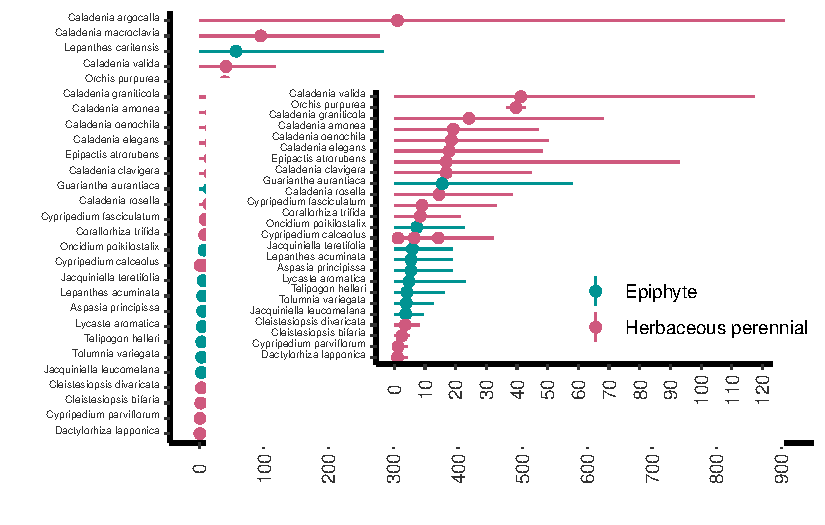
\includegraphics{121-Rage_Largo_y_Expectativa_de_Vida_files/figure-pdf/LV8-1.pdf}

Lo más importante de esta figura es notar las gran incertidumbre que hay
en los estimados de la esperanza de vida, lo cual se refleja en los
intervalos de confianza. Esta incertidumbre puede deberse a varios
factores, como la calidad de los datos, la variabilidad biológica entre
individuos y poblaciones, y las limitaciones inherentes a los modelos
utilizados para estimar la esperanza de vida a partir de matrices de
transición.

Posterior a este análisis es importante regresar a cada
modelo/especie/población y evaluar la calidad de los datos y los
supuestos del modelo para entender mejor las fuentes de incertidumbre y
cómo podrían ser mitigadas en futuros estudios. Claramente hay unas
especies donde los estimados paraceen más confiables que en otras. En
adición hay algunas especies donde el la esperanza de vida parace
completamente irreal, lo cual sugiere que hay problemas con los datos o
el modelo para esas especies en particular.

\begin{center}\rule{0.5\linewidth}{0.5pt}\end{center}

\begin{center}\rule{0.5\linewidth}{0.5pt}\end{center}

\section{Longevidad de vida}\label{longevidad-de-vida}

\begin{Shaded}
\begin{Highlighting}[]
\CommentTok{\#index\_O\_calculado \textless{}{-} index\_O\_filtrado\_final \%\textgreater{}\%}
\CommentTok{\#  mutate(life\_expectancy = mapply(lifeExpectancy, matU, start\_life)) \%\textgreater{}\% \# calcular el largo de vida promedio}
\CommentTok{\#  mutate(var\_life\_expectancy = mapply(life\_expect\_var, matU, start = 1)) \%\textgreater{}\% \# calcular la varianza del largo de vida}
\CommentTok{\#  mutate(low\_CI\_var\_LS = pmax(0, life\_expectancy {-} 1.96 * sqrt(var\_life\_expectancy))) \%\textgreater{}\% \# calcular el intervalo de confianza inferior}
\CommentTok{\#  mutate(high\_CI\_var\_LS = life\_expectancy + 1.96 * sqrt(var\_life\_expectancy)) \%\textgreater{}\% \# calcular el intervalo de confianza superior}
\CommentTok{\#  mutate(OrganismType = reorder(OrganismType, life\_expectancy, median)) \# ordenar las especies por el largo de vida }




\NormalTok{index\_O\_filtrado\_final }\SpecialCharTok{\%\textgreater{}\%}
  \FunctionTok{mutate}\NormalTok{(}
    \AttributeTok{life\_expectancy =} \FunctionTok{mapply}\NormalTok{(lifeExpectancy, matU, start\_life),}
    \AttributeTok{var\_life\_expectancy =} \FunctionTok{mapply}\NormalTok{(life\_expect\_var, matU, }\AttributeTok{start =} \DecValTok{1}\NormalTok{)}
\NormalTok{  ) }\SpecialCharTok{\%\textgreater{}\%}
  \FunctionTok{group\_by}\NormalTok{(Species) }\SpecialCharTok{\%\textgreater{}\%}
  \FunctionTok{summarise}\NormalTok{(}
    \AttributeTok{Q1\_life\_expectancy =} \FunctionTok{quantile}\NormalTok{(life\_expectancy, }\FloatTok{0.25}\NormalTok{, }\AttributeTok{na.rm =} \ConstantTok{TRUE}\NormalTok{),}
    \AttributeTok{Median\_life\_expectancy =} \FunctionTok{quantile}\NormalTok{(life\_expectancy, }\FloatTok{0.5}\NormalTok{, }\AttributeTok{na.rm =} \ConstantTok{TRUE}\NormalTok{),}
    \AttributeTok{Q3\_life\_expectancy =} \FunctionTok{quantile}\NormalTok{(life\_expectancy, }\FloatTok{0.75}\NormalTok{, }\AttributeTok{na.rm =} \ConstantTok{TRUE}\NormalTok{),}
    \AttributeTok{.groups =} \StringTok{"drop"}
\NormalTok{  )}






\NormalTok{index\_O\_calculado\_median }\OtherTok{\textless{}{-}}\NormalTok{ index\_O\_filtrado\_final }\SpecialCharTok{\%\textgreater{}\%}
  \FunctionTok{mutate}\NormalTok{(}\AttributeTok{life\_expectancy =} \FunctionTok{mapply}\NormalTok{(lifeExpectancy, matU, start\_life)) }\SpecialCharTok{\%\textgreater{}\%}
  \FunctionTok{mutate}\NormalTok{(}\AttributeTok{var\_life\_expectancy =} \FunctionTok{mapply}\NormalTok{(life\_expect\_var, matU, }\AttributeTok{start =} \DecValTok{1}\NormalTok{)) }\SpecialCharTok{\%\textgreater{}\%}
  \FunctionTok{group\_by}\NormalTok{(SpeciesAccepted) }\SpecialCharTok{\%\textgreater{}\%}
  \FunctionTok{mutate}\NormalTok{(}
    \AttributeTok{Q1\_life\_expectancy =} \FunctionTok{quantile}\NormalTok{(life\_expectancy, }\FloatTok{0.25}\NormalTok{, }\AttributeTok{na.rm =} \ConstantTok{TRUE}\NormalTok{),}
    \AttributeTok{Median\_life\_expectancy =} \FunctionTok{quantile}\NormalTok{(life\_expectancy, }\FloatTok{0.5}\NormalTok{, }\AttributeTok{na.rm =} \ConstantTok{TRUE}\NormalTok{),}
    \AttributeTok{Q3\_life\_expectancy =} \FunctionTok{quantile}\NormalTok{(life\_expectancy, }\FloatTok{0.75}\NormalTok{, }\AttributeTok{na.rm =} \ConstantTok{TRUE}\NormalTok{)}
\NormalTok{  ) }\SpecialCharTok{\%\textgreater{}\%}
  \FunctionTok{ungroup}\NormalTok{() }\SpecialCharTok{\%\textgreater{}\%}
  \FunctionTok{mutate}\NormalTok{(}\AttributeTok{OrganismType =} \FunctionTok{reorder}\NormalTok{(OrganismType, life\_expectancy, median))}

\NormalTok{index\_O\_calculado\_subset2}\OtherTok{=}\NormalTok{index\_O\_calculado\_median }\SpecialCharTok{|\textgreater{}} 
  \FunctionTok{select}\NormalTok{(mat, SpeciesAccepted, OrganismType, life\_expectancy, Q1\_life\_expectancy, }
\NormalTok{         Q3\_life\_expectancy, Median\_life\_expectancy) }\SpecialCharTok{|\textgreater{}} 
  \FunctionTok{mutate}\NormalTok{(}\AttributeTok{OrganismType\_RC=}\FunctionTok{fct\_recode}\NormalTok{(OrganismType,}
                             \StringTok{"Epífita"}\OtherTok{=}\StringTok{"Epiphyte"}\NormalTok{,}
                             \StringTok{"Terrestre"}\OtherTok{=}\StringTok{"Herbaceous perennial"}\NormalTok{))}


\NormalTok{index\_O\_calculado\_subset2}\SpecialCharTok{$}\NormalTok{SpeciesAccepted }\OtherTok{\textless{}{-}} \FunctionTok{fct\_reorder}\NormalTok{(}
\NormalTok{  index\_O\_calculado\_subset2}\SpecialCharTok{$}\NormalTok{SpeciesAccepted,}
\NormalTok{  index\_O\_calculado\_subset2}\SpecialCharTok{$}\NormalTok{Median\_life\_expectancy,}
  \AttributeTok{.desc =} \ConstantTok{FALSE}
\NormalTok{)}


\NormalTok{main.plot\_median }\OtherTok{\textless{}{-}} \FunctionTok{ggplot}\NormalTok{(index\_O\_calculado\_subset2, }\FunctionTok{aes}\NormalTok{(SpeciesAccepted, }\AttributeTok{color =}\NormalTok{ OrganismType\_RC)) }\SpecialCharTok{+}
  \FunctionTok{geom\_linerange}\NormalTok{(}\FunctionTok{aes}\NormalTok{(}\AttributeTok{x =}\NormalTok{ SpeciesAccepted, }\AttributeTok{ymin =}\NormalTok{ Q1\_life\_expectancy, }\AttributeTok{ymax =}\NormalTok{ Q3\_life\_expectancy)) }\SpecialCharTok{+}
  \FunctionTok{geom\_point}\NormalTok{(}\FunctionTok{aes}\NormalTok{(}\AttributeTok{y =}\NormalTok{ Median\_life\_expectancy), }\AttributeTok{size =} \DecValTok{2}\NormalTok{) }\SpecialCharTok{+}
  \FunctionTok{coord\_flip}\NormalTok{() }\SpecialCharTok{+}
  \FunctionTok{theme}\NormalTok{(}\AttributeTok{legend.position.inside =} \FunctionTok{c}\NormalTok{(}\FloatTok{0.8}\NormalTok{, }\FloatTok{0.2}\NormalTok{))}



\NormalTok{main.plot\_median}
\end{Highlighting}
\end{Shaded}

\begin{center}\rule{0.5\linewidth}{0.5pt}\end{center}

\section{Longevidad sin los intervalos de
confianza}\label{longevidad-sin-los-intervalos-de-confianza}

La longevidad es el largo de vida máximo que puede alcanzar un individuo
en una población. En este caso se usa la función \textbf{longevity} para
calcular el tiempo para un cohorte llegue a un 5\% de supervivencia. La
función \textbf{longevity} requiere la matriz de transición
\textbf{matU} y la etapa de inicio de la vida \textbf{start\_life}.

\begin{Shaded}
\begin{Highlighting}[]
\CommentTok{\# names(index\_O\_calculado)}

\NormalTok{index\_O\_calculado\_subset}\OtherTok{=}\NormalTok{index\_O\_calculado }\SpecialCharTok{|\textgreater{}} 
  \FunctionTok{select}\NormalTok{(mat, SpeciesAccepted, OrganismType, life\_expectancy, var\_life\_expectancy, }
\NormalTok{         low\_CI\_var\_LS, high\_CI\_var\_LS, OrganismType) }\SpecialCharTok{|\textgreater{}} 
  \FunctionTok{mutate}\NormalTok{(}\AttributeTok{OrganismType\_RC=}\FunctionTok{fct\_recode}\NormalTok{(OrganismType,}
                             \StringTok{"Epífita"}\OtherTok{=}\StringTok{"Epiphyte"}\NormalTok{,}
                             \StringTok{"Terrestre"}\OtherTok{=}\StringTok{"Herbaceous perennial"}\NormalTok{))}


\NormalTok{longevity\_O }\OtherTok{\textless{}{-}}\NormalTok{ index\_O\_filtrado\_final }\SpecialCharTok{\%\textgreater{}\%}
  \FunctionTok{mutate}\NormalTok{(}\AttributeTok{longevidad1=}\FunctionTok{mapply}\NormalTok{(longevity, matU, }\AttributeTok{start =} \DecValTok{1}\NormalTok{, }\AttributeTok{lx\_crit =} \FloatTok{0.05}\NormalTok{),}
         \AttributeTok{longevidad2=}\FunctionTok{mapply}\NormalTok{(longevity, matU, }\AttributeTok{start =} \DecValTok{2}\NormalTok{, }\AttributeTok{lx\_crit =} \FloatTok{0.05}\NormalTok{)) }\CommentTok{\# calcular la longevidad por cada especie}
\end{Highlighting}
\end{Shaded}

\begin{Shaded}
\begin{Highlighting}[]
\CommentTok{\#names(longevity\_O)}

\NormalTok{index\_O\_filtrado\_final }\OtherTok{\textless{}{-}}\NormalTok{ index\_O\_filtrado }\SpecialCharTok{\%\textgreater{}\%}
  \FunctionTok{filter}\NormalTok{(}\FunctionTok{sapply}\NormalTok{(matU, }\ControlFlowTok{function}\NormalTok{(mat) \{}
    \ControlFlowTok{if}\NormalTok{ (}\FunctionTok{is.null}\NormalTok{(mat)) }\FunctionTok{return}\NormalTok{(}\ConstantTok{FALSE}\NormalTok{)}
    \FunctionTok{all}\NormalTok{(}\FunctionTok{colSums}\NormalTok{(mat, }\AttributeTok{na.rm =} \ConstantTok{TRUE}\NormalTok{) }\SpecialCharTok{\textless{}=} \DecValTok{1}\NormalTok{)}
\NormalTok{  \}))}


\NormalTok{longevity\_O }\OtherTok{\textless{}{-}}\NormalTok{ index\_O\_filtrado\_final }\SpecialCharTok{\%\textgreater{}\%}
  \FunctionTok{mutate}\NormalTok{(}\AttributeTok{longevidad1=}\FunctionTok{mapply}\NormalTok{(longevity, matU, }\AttributeTok{start =} \DecValTok{1}\NormalTok{, }\AttributeTok{lx\_crit =} \FloatTok{0.05}\NormalTok{),}
         \AttributeTok{longevidad2=}\FunctionTok{mapply}\NormalTok{(longevity, matU, }\AttributeTok{start =} \DecValTok{2}\NormalTok{, }\AttributeTok{lx\_crit =} \FloatTok{0.05}\NormalTok{)) }\CommentTok{\# calcular la longevidad por cada especie}


\NormalTok{longevity\_O}\OtherTok{=}\NormalTok{longevity\_O}\SpecialCharTok{|\textgreater{}}
\FunctionTok{mutate}\NormalTok{(}\AttributeTok{OrganismType\_RC=}\FunctionTok{fct\_recode}\NormalTok{(OrganismType,}
                            \StringTok{"Epífita"}\OtherTok{=}\StringTok{"Epiphyte"}\NormalTok{,}
                            \StringTok{"Terrestre"}\OtherTok{=}\StringTok{"Herbaceous perennial"}\NormalTok{))}

\NormalTok{longevity\_O}\SpecialCharTok{$}\NormalTok{SpeciesAccepted }\OtherTok{\textless{}{-}} \FunctionTok{fct\_reorder}\NormalTok{(}
\NormalTok{  longevity\_O}\SpecialCharTok{$}\NormalTok{SpeciesAccepted,}
\NormalTok{  longevity\_O}\SpecialCharTok{$}\NormalTok{longevidad1,}
  \AttributeTok{.desc =} \ConstantTok{FALSE}
\NormalTok{)}

\NormalTok{main.plot}\OtherTok{=}\FunctionTok{ggplot}\NormalTok{(longevity\_O , }\FunctionTok{aes}\NormalTok{(}\AttributeTok{x=}\NormalTok{SpeciesAccepted, }\AttributeTok{y=}\NormalTok{longevidad2, }\AttributeTok{color =}\NormalTok{ OrganismType\_RC)) }\SpecialCharTok{+}
  \FunctionTok{geom\_point}\NormalTok{() }\SpecialCharTok{+}
 \FunctionTok{coord\_flip}\NormalTok{() }\SpecialCharTok{+}
  \FunctionTok{theme}\NormalTok{(}\AttributeTok{legend.position.inside =} \FunctionTok{c}\NormalTok{(}\FloatTok{0.8}\NormalTok{, }\FloatTok{0.2}\NormalTok{)) }\SpecialCharTok{+}
  \FunctionTok{ylab}\NormalTok{(}\StringTok{""}\NormalTok{) }\SpecialCharTok{+}
  \FunctionTok{xlab}\NormalTok{(}\StringTok{""}\NormalTok{) }\SpecialCharTok{+}
  \FunctionTok{rlt\_style\_colour}\NormalTok{() }\SpecialCharTok{+}
  \FunctionTok{theme}\NormalTok{(}
    \AttributeTok{axis.text.x =} \FunctionTok{element\_text}\NormalTok{(}
      \AttributeTok{color =} \StringTok{"grey20"}\NormalTok{,}
      \AttributeTok{size =} \DecValTok{9}\NormalTok{,}
      \AttributeTok{angle =} \DecValTok{90}\NormalTok{,}
      \AttributeTok{hjust =}\NormalTok{ .}\DecValTok{5}\NormalTok{,}
      \AttributeTok{vjust =}\NormalTok{ .}\DecValTok{5}\NormalTok{,}
      \AttributeTok{face =} \StringTok{"plain"}
\NormalTok{    ),}
    \AttributeTok{axis.text.y =} \FunctionTok{element\_text}\NormalTok{(}
      \AttributeTok{color =} \StringTok{"grey20"}\NormalTok{,}
      \AttributeTok{size =} \DecValTok{7}\NormalTok{,}
      \AttributeTok{angle =} \DecValTok{0}\NormalTok{,}
      \AttributeTok{hjust =} \DecValTok{1}\NormalTok{,}
      \AttributeTok{vjust =} \DecValTok{0}\NormalTok{,}
      \AttributeTok{face =} \StringTok{"plain"}
\NormalTok{    ),}
    \AttributeTok{axis.title.x =} \FunctionTok{element\_text}\NormalTok{(}
      \AttributeTok{color =} \StringTok{"grey20"}\NormalTok{,}
      \AttributeTok{size =} \DecValTok{12}\NormalTok{,}
      \AttributeTok{angle =} \DecValTok{0}\NormalTok{,}
      \AttributeTok{hjust =}\NormalTok{ .}\DecValTok{5}\NormalTok{,}
      \AttributeTok{vjust =} \DecValTok{0}\NormalTok{,}
      \AttributeTok{face =} \StringTok{"plain"}
\NormalTok{    ),}
    \AttributeTok{axis.title.y =} \FunctionTok{element\_text}\NormalTok{(}
      \AttributeTok{color =} \StringTok{"grey20"}\NormalTok{,}
      \AttributeTok{size =} \DecValTok{12}\NormalTok{,}
      \AttributeTok{angle =} \DecValTok{90}\NormalTok{,}
      \AttributeTok{hjust =}\NormalTok{ .}\DecValTok{5}\NormalTok{,}
      \AttributeTok{vjust =}\NormalTok{ .}\DecValTok{5}\NormalTok{,}
      \AttributeTok{face =} \StringTok{"plain"}
\NormalTok{    )}
\NormalTok{  )}\SpecialCharTok{+}
  \FunctionTok{theme}\NormalTok{(}\AttributeTok{legend.position=}\StringTok{"none"}\NormalTok{)}\SpecialCharTok{+}
  \FunctionTok{theme}\NormalTok{(}\AttributeTok{axis.text.y =} \FunctionTok{element\_text}\NormalTok{(}\AttributeTok{size =} \DecValTok{5}\NormalTok{))}\SpecialCharTok{+}
  \FunctionTok{scale\_y\_continuous}\NormalTok{(}\AttributeTok{n.breaks =} \DecValTok{12}\NormalTok{)}

\DocumentationTok{\#\# Insertar la figura con las especies con longevidad \textless{}50 años}

\NormalTok{inset.plot}\OtherTok{=}\NormalTok{longevity\_O }\SpecialCharTok{|\textgreater{}} 
  \FunctionTok{filter}\NormalTok{(longevidad2 }\SpecialCharTok{\textless{}}\DecValTok{50}\NormalTok{) }\SpecialCharTok{|\textgreater{}} 
\FunctionTok{ggplot}\NormalTok{(}\FunctionTok{aes}\NormalTok{(}\AttributeTok{x=}\NormalTok{SpeciesAccepted, }\AttributeTok{y=}\NormalTok{longevidad2, }\AttributeTok{color =}\NormalTok{ OrganismType\_RC)) }\SpecialCharTok{+}
  \FunctionTok{geom\_point}\NormalTok{() }\SpecialCharTok{+}
  \FunctionTok{coord\_flip}\NormalTok{() }\SpecialCharTok{+}
  \FunctionTok{theme}\NormalTok{(}\AttributeTok{legend.position.inside =} \FunctionTok{c}\NormalTok{(}\FloatTok{0.8}\NormalTok{, }\FloatTok{0.2}\NormalTok{)) }\SpecialCharTok{+}
  \FunctionTok{ylab}\NormalTok{(}\StringTok{""}\NormalTok{) }\SpecialCharTok{+}
  \FunctionTok{xlab}\NormalTok{(}\StringTok{""}\NormalTok{) }\SpecialCharTok{+}
  \FunctionTok{rlt\_style\_colour}\NormalTok{() }\SpecialCharTok{+}
  \FunctionTok{theme}\NormalTok{(}
    \AttributeTok{axis.text.x =} \FunctionTok{element\_text}\NormalTok{(}
      \AttributeTok{color =} \StringTok{"grey20"}\NormalTok{,}
      \AttributeTok{size =} \DecValTok{9}\NormalTok{,}
      \AttributeTok{angle =} \DecValTok{90}\NormalTok{,}
      \AttributeTok{hjust =}\NormalTok{ .}\DecValTok{5}\NormalTok{,}
      \AttributeTok{vjust =}\NormalTok{ .}\DecValTok{5}\NormalTok{,}
      \AttributeTok{face =} \StringTok{"plain"}
\NormalTok{    ),}
    \AttributeTok{axis.text.y =} \FunctionTok{element\_text}\NormalTok{(}
      \AttributeTok{color =} \StringTok{"grey20"}\NormalTok{,}
      \AttributeTok{size =} \DecValTok{7}\NormalTok{,}
      \AttributeTok{angle =} \DecValTok{0}\NormalTok{,}
      \AttributeTok{hjust =} \DecValTok{1}\NormalTok{,}
      \AttributeTok{vjust =} \DecValTok{0}\NormalTok{,}
      \AttributeTok{face =} \StringTok{"plain"}
\NormalTok{    ),}
    \AttributeTok{axis.title.x =} \FunctionTok{element\_text}\NormalTok{(}
      \AttributeTok{color =} \StringTok{"grey20"}\NormalTok{,}
      \AttributeTok{size =} \DecValTok{12}\NormalTok{,}
      \AttributeTok{angle =} \DecValTok{0}\NormalTok{,}
      \AttributeTok{hjust =}\NormalTok{ .}\DecValTok{5}\NormalTok{,}
      \AttributeTok{vjust =} \DecValTok{0}\NormalTok{,}
      \AttributeTok{face =} \StringTok{"plain"}
\NormalTok{    ),}
    \AttributeTok{axis.title.y =} \FunctionTok{element\_text}\NormalTok{(}
      \AttributeTok{color =} \StringTok{"grey20"}\NormalTok{,}
      \AttributeTok{size =} \DecValTok{12}\NormalTok{,}
      \AttributeTok{angle =} \DecValTok{90}\NormalTok{,}
      \AttributeTok{hjust =}\NormalTok{ .}\DecValTok{5}\NormalTok{,}
      \AttributeTok{vjust =}\NormalTok{ .}\DecValTok{5}\NormalTok{,}
      \AttributeTok{face =} \StringTok{"plain"}
\NormalTok{    )}
\NormalTok{  )}\SpecialCharTok{+}
  \FunctionTok{theme}\NormalTok{(}\AttributeTok{legend.position =} \FunctionTok{c}\NormalTok{(}\FloatTok{0.8}\NormalTok{,}\FloatTok{0.2}\NormalTok{),}
        \AttributeTok{legend.title =} \FunctionTok{element\_blank}\NormalTok{())}\SpecialCharTok{+}
  \FunctionTok{theme}\NormalTok{(}\AttributeTok{axis.text.y =} \FunctionTok{element\_text}\NormalTok{(}\AttributeTok{size =} \DecValTok{5}\NormalTok{))}\SpecialCharTok{+}
  \FunctionTok{scale\_y\_continuous}\NormalTok{(}\AttributeTok{n.breaks =} \DecValTok{12}\NormalTok{)}

\FunctionTok{library}\NormalTok{(cowplot)}

\NormalTok{longevidad\_plot }\OtherTok{\textless{}{-}} \FunctionTok{ggdraw}\NormalTok{() }\SpecialCharTok{+}
  \FunctionTok{draw\_plot}\NormalTok{(main.plot) }\SpecialCharTok{+}
  \FunctionTok{draw\_plot}\NormalTok{(inset.plot, }\AttributeTok{x =} \FloatTok{0.3}\NormalTok{, }\AttributeTok{y =} \FloatTok{0.15}\NormalTok{, }\AttributeTok{width =} \FloatTok{0.7}\NormalTok{, }\AttributeTok{height =} \FloatTok{0.7}\NormalTok{)}

\NormalTok{longevidad\_plot}
\end{Highlighting}
\end{Shaded}

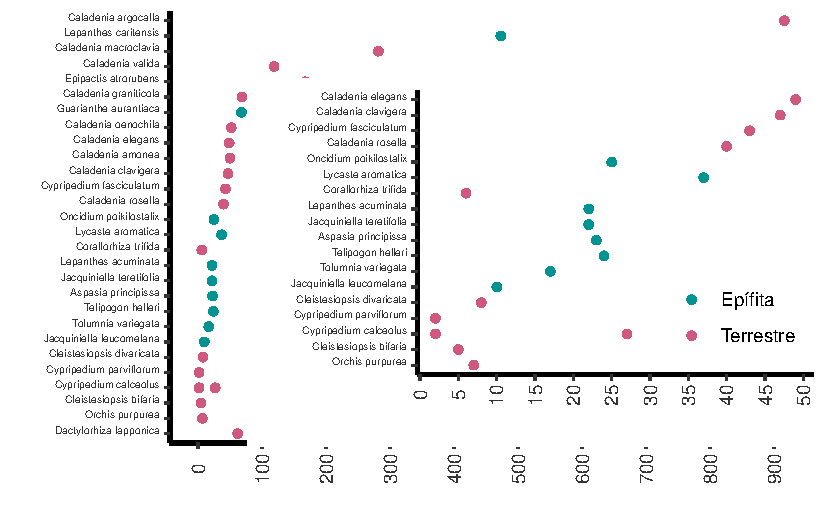
\includegraphics{121-Rage_Largo_y_Expectativa_de_Vida_files/figure-pdf/LV12-1.pdf}

\subsubsection{}\label{section}

Estimar el largo de

Figura del largo de vida promedio y su varianza para las orquídeas
terrestres y epifitas.

\begin{Shaded}
\begin{Highlighting}[]
\NormalTok{lifeExpectancy }\OtherTok{\textless{}{-}} \ControlFlowTok{function}\NormalTok{(matU, startLife) \{}
\NormalTok{  N }\OtherTok{\textless{}{-}} \FunctionTok{solve}\NormalTok{(}\FunctionTok{diag}\NormalTok{(}\FunctionTok{nrow}\NormalTok{(matU)) }\SpecialCharTok{{-}}\NormalTok{ matU)}
  \FunctionTok{return}\NormalTok{(}\FunctionTok{colSums}\NormalTok{(N)[startLife])}
\NormalTok{\}}


\NormalTok{compadre\_life\_expect }\OtherTok{\textless{}{-}}\NormalTok{ Orquideas }\SpecialCharTok{\%\textgreater{}\%}
  \FunctionTok{filter}\NormalTok{(ProjectionInterval }\SpecialCharTok{==} \FloatTok{1.0}\NormalTok{) }\SpecialCharTok{|\textgreater{}} \CommentTok{\# filtrar para matriz de un año solamente}
  \FunctionTok{filter}\NormalTok{(}
\NormalTok{    MatrixComposite }\SpecialCharTok{==} \StringTok{"Mean"}\NormalTok{, }\CommentTok{\# filtrar para la matriz promedia}
\NormalTok{    MatrixTreatment }\SpecialCharTok{==} \StringTok{"Unmanipulated"}\NormalTok{, }\CommentTok{\# filtrar para la matriz sin manipulación}
\NormalTok{    MatrixCaptivity }\SpecialCharTok{==} \StringTok{"W"} \CommentTok{\# filtrar para poblaciones naturales (no en cautiverio)}
\NormalTok{  ) }\SpecialCharTok{\%\textgreater{}\%}
  \FunctionTok{mutate}\NormalTok{(}\AttributeTok{StageID =} \FunctionTok{cdb\_id\_stages}\NormalTok{(.)) }\SpecialCharTok{\%\textgreater{}\%} \CommentTok{\# crear un ID para las etapas}
  \FunctionTok{cdb\_collapse}\NormalTok{(}\AttributeTok{columns =} \StringTok{"StageID"}\NormalTok{) }\SpecialCharTok{\%\textgreater{}\%} \CommentTok{\# colapsar las etapas}
  \FunctionTok{cdb\_flag}\NormalTok{() }\SpecialCharTok{\%\textgreater{}\%} \CommentTok{\# evaluar las matrices y crear una columna para cada evaluación}
  \FunctionTok{filter}\NormalTok{(}
\NormalTok{    check\_NA\_U }\SpecialCharTok{==} \ConstantTok{FALSE}\NormalTok{, }\CommentTok{\# filtrar para matrices sin valores faltantes}
\NormalTok{    check\_zero\_U }\SpecialCharTok{==} \ConstantTok{FALSE}\NormalTok{, }\CommentTok{\# filtrar para matrices sin valores cero}
\NormalTok{    check\_singular\_U }\SpecialCharTok{==} \ConstantTok{FALSE}\NormalTok{,}
\NormalTok{    check\_surv\_gte\_1 }\SpecialCharTok{==} \ConstantTok{FALSE}\NormalTok{, }\CommentTok{\# filtrar para matrices sin valores de supervivencia mayores a 1}
\NormalTok{  ) }\SpecialCharTok{\%\textgreater{}\%} \CommentTok{\# filtrar para matrices no singulares}
  \FunctionTok{mutate}\NormalTok{(}\AttributeTok{matU =} \FunctionTok{matU}\NormalTok{(.), }\AttributeTok{start\_life =} \FunctionTok{mpm\_first\_active}\NormalTok{(.)) }\SpecialCharTok{\%\textgreater{}\%} \CommentTok{\# extraer la matriz de transición y la etapa de inicio de la vida}
  \FunctionTok{mutate}\NormalTok{(}\AttributeTok{life\_expectancy =} \FunctionTok{mapply}\NormalTok{(lifeExpectancy, matU, start\_life)) }\SpecialCharTok{\%\textgreater{}\%} \CommentTok{\# calcular el largo de vida}
  \FunctionTok{mutate}\NormalTok{(}\AttributeTok{var\_life\_expectancy =} \FunctionTok{mapply}\NormalTok{(life\_expect\_var, matU, }\AttributeTok{start =} \DecValTok{1}\NormalTok{)) }\SpecialCharTok{\%\textgreater{}\%} \CommentTok{\# calcular la varianza del largo de vida}
  \FunctionTok{mutate}\NormalTok{(}\AttributeTok{low\_CI\_var\_LS =}\NormalTok{ life\_expectancy }\SpecialCharTok{{-}} \FloatTok{1.96} \SpecialCharTok{*} \FunctionTok{sqrt}\NormalTok{(var\_life\_expectancy)) }\SpecialCharTok{\%\textgreater{}\%} \CommentTok{\# calcular el intervalo de confianza inferior}
  \FunctionTok{mutate}\NormalTok{(}
    \AttributeTok{high\_CI\_var\_LS =}\NormalTok{ life\_expectancy }\SpecialCharTok{+} \FloatTok{1.96} \SpecialCharTok{*} \FunctionTok{sqrt}\NormalTok{(var\_life\_expectancy)) }\SpecialCharTok{\%\textgreater{}\%} \CommentTok{\# calcular el intervalo de confianza superior}
  \FunctionTok{mutate}\NormalTok{(}\AttributeTok{OrganismType =} \FunctionTok{reorder}\NormalTok{(OrganismType, life\_expectancy, median)) }\CommentTok{\# ordenar las especies por el largo de vida}
\end{Highlighting}
\end{Shaded}

Visualizar el largo de vida por plantas epifitas versus terrestres. Nota
aquí que algunas especies están representada múltiple veces. Por
consecuencia la distribución de los datos no es una buena representación
de la diferencia entre las especies epifitas y terrestres, debido a lo
que se llama pseudoreplicación. Este tabla representa la distribución
los datos del data frame anterior.

Calculando el promedio y la desviación estándar de la esperanza de vida
de las orquídeas.

\begin{Shaded}
\begin{Highlighting}[]
\NormalTok{index\_O\_calculado }\SpecialCharTok{|\textgreater{}}
  \FunctionTok{group\_by}\NormalTok{(OrganismType) }\SpecialCharTok{|\textgreater{}}
  \FunctionTok{summarize}\NormalTok{(}
    \AttributeTok{mean\_LS =} \FunctionTok{mean}\NormalTok{(life\_expectancy, }\AttributeTok{na.rm =} \ConstantTok{TRUE}\NormalTok{),}
    \AttributeTok{sd\_LS =} \FunctionTok{sd}\NormalTok{(var\_life\_expectancy, }\AttributeTok{na.rm =} \ConstantTok{TRUE}\NormalTok{)}
\NormalTok{  )}


\CommentTok{\#OrchidLS |\textgreater{}}
\CommentTok{\#  group\_by(OrganismType) |\textgreater{}}
\CommentTok{\#  summarize(}
 \CommentTok{\#   mean\_LS = mean(life\_expectancy, na.rm = TRUE),}
 \CommentTok{\#   sd\_LS = sd(life\_expectancy, na.rm = TRUE)}
\CommentTok{\#  )}
\end{Highlighting}
\end{Shaded}

Haciendo una figura del largo de vida de las especies epífitas y
terrestres. Nota que la escala es logarítmica.

\begin{Shaded}
\begin{Highlighting}[]
\NormalTok{ggplot2}\SpecialCharTok{::}\FunctionTok{ggplot}\NormalTok{(}
\NormalTok{  index\_O\_calculado,}
  \FunctionTok{aes}\NormalTok{(OrganismType, life\_expectancy, }\AttributeTok{colour =}\NormalTok{ OrganismType)}
\NormalTok{) }\SpecialCharTok{+}
  \FunctionTok{geom\_boxplot}\NormalTok{(}\AttributeTok{size=}\NormalTok{.}\DecValTok{8}\NormalTok{) }\SpecialCharTok{+}
  \FunctionTok{geom\_point}\NormalTok{() }\SpecialCharTok{+}
  \FunctionTok{scale\_y\_log10}\NormalTok{() }\SpecialCharTok{+}
  \FunctionTok{coord\_flip}\NormalTok{() }\SpecialCharTok{+}
  \FunctionTok{labs}\NormalTok{(}\AttributeTok{x =} \ConstantTok{NULL}\NormalTok{, }\AttributeTok{y =} \StringTok{"Life expectancy (log(years))"}\NormalTok{) }\SpecialCharTok{+}
\NormalTok{  rlt\_theme }\SpecialCharTok{+}
  \FunctionTok{theme}\NormalTok{(}\AttributeTok{legend.position =} \StringTok{"none"}\NormalTok{)}

\FunctionTok{ggsave}\NormalTok{(}\StringTok{"Figures/Life\_Span.png"}\NormalTok{)}
\end{Highlighting}
\end{Shaded}

https://jonesor.github.io/Rage/reference/life\_expect.html

En el siguiente script y gráfico vemos la visualización por genero de
los estimados de la esperanza de vida. Nota que la esperanza de vida es
un estimado y no un valor exacto. En este caso se usa la función
\textbf{life\_expect\_var} para calcular la varianza de la esperanza de
vida. La escala de x (el largo de vida fue cambiado a log10 de la
esperanza de vida).

\textbf{How to calculate CI of life span, it is in the table above, use
gamma, not normal} !!!!

low\_CI\_var\_LS high\_CI\_var\_LS

\begin{Shaded}
\begin{Highlighting}[]
\CommentTok{\#SPECIES\_O$SpeciesAccepted \textless{}{-} fct\_reorder(SPECIES\_O$SpeciesAccepted, SPECIES\_O$StudyStart, .desc = FALSE) \# Ordenar por fecha de inicio del estudio}


\FunctionTok{ggplot}\NormalTok{(}
\NormalTok{  index\_O\_calculado,}
  \FunctionTok{aes}\NormalTok{(}
    \AttributeTok{x =} \FunctionTok{reorder}\NormalTok{(SpeciesAccepted, life\_expectancy),}
\NormalTok{    life\_expectancy,}
    \AttributeTok{colour =}\NormalTok{ OrganismType}
\NormalTok{  )}
\NormalTok{) }\SpecialCharTok{+}
  \CommentTok{\# geom\_boxplot() +}
  \FunctionTok{geom\_point}\NormalTok{() }\SpecialCharTok{+}
  \FunctionTok{scale\_y\_log10}\NormalTok{() }\SpecialCharTok{+}
  \FunctionTok{coord\_flip}\NormalTok{() }\SpecialCharTok{+}
  \FunctionTok{labs}\NormalTok{(}\AttributeTok{x =} \ConstantTok{NULL}\NormalTok{, }\AttributeTok{y =} \StringTok{"Life expectancy (log(years))"}\NormalTok{)}
\CommentTok{\#  rlt\_theme+}
\CommentTok{\#theme(legend.position = "none")}

\CommentTok{\#ggsave("Figures/Genus\_Life\_Span.png")}
\end{Highlighting}
\end{Shaded}

EWl largo de vida de las Caladenia solamente

Evaluando el largo de vida de las especies de \emph{Caladenia} solamente

\begin{Shaded}
\begin{Highlighting}[]
\CommentTok{\#SPECIES\_O$SpeciesAccepted \textless{}{-} fct\_reorder(SPECIES\_O$SpeciesAccepted, SPECIES\_O$StudyStart, .desc = FALSE)}

\NormalTok{index\_O\_calculado }\SpecialCharTok{|\textgreater{}}
  \FunctionTok{group\_by}\NormalTok{(Genus) }\SpecialCharTok{|\textgreater{}}
  \FunctionTok{summarize}\NormalTok{(}
    \AttributeTok{mean\_LS =} \FunctionTok{mean}\NormalTok{(life\_expectancy, }\AttributeTok{na.rm =} \ConstantTok{TRUE}\NormalTok{),}
    \AttributeTok{sd\_LS =} \FunctionTok{sd}\NormalTok{(life\_expectancy, }\AttributeTok{na.rm =} \ConstantTok{TRUE}\NormalTok{)}
\NormalTok{  ) }\SpecialCharTok{|\textgreater{}}
  \FunctionTok{filter}\NormalTok{(Genus }\SpecialCharTok{\%in\%} \FunctionTok{c}\NormalTok{(}\StringTok{"Caladenia"}\NormalTok{))}

\NormalTok{index\_O\_calculado }\SpecialCharTok{|\textgreater{}}
  \FunctionTok{filter}\NormalTok{(Genus }\SpecialCharTok{\%in\%} \FunctionTok{c}\NormalTok{(}\StringTok{"Caladenia"}\NormalTok{)) }\SpecialCharTok{|\textgreater{}}
  \FunctionTok{ggplot}\NormalTok{(}\FunctionTok{aes}\NormalTok{(}
    \AttributeTok{x =} \FunctionTok{reorder}\NormalTok{(SpeciesAccepted, life\_expectancy),}
\NormalTok{    life\_expectancy,}
    \AttributeTok{colour =}\NormalTok{ OrganismType}
\NormalTok{  )) }\SpecialCharTok{+}
  \FunctionTok{geom\_point}\NormalTok{() }\SpecialCharTok{+}
  \FunctionTok{scale\_y\_log10}\NormalTok{() }\SpecialCharTok{+}
  \FunctionTok{coord\_flip}\NormalTok{() }\SpecialCharTok{+}
  \FunctionTok{labs}\NormalTok{(}\AttributeTok{x =} \ConstantTok{NULL}\NormalTok{, }\AttributeTok{y =} \StringTok{"Life expectancy (years)"}\NormalTok{) }\SpecialCharTok{+}
\NormalTok{  rlt\_theme }\SpecialCharTok{+}
  \FunctionTok{theme}\NormalTok{(}\AttributeTok{legend.position =} \StringTok{"none"}\NormalTok{)}

\CommentTok{\#ggsave("Figures/Caladenia\_Life\_Span.png")}
\end{Highlighting}
\end{Shaded}

https://jonesor.github.io/Rage/articles/a03\_LifeHistoryTraits.html

\section{Reproducción y
maduración}\label{reproducciuxf3n-y-maduraciuxf3n}

\section{Caracteristicas de componentes de tabla de
vida}\label{caracteristicas-de-componentes-de-tabla-de-vida}

\section{La distribución de mortandad y
fecundidad}\label{la-distribuciuxf3n-de-mortandad-y-fecundidad}

Baudisch, A. 2011. The pace and shape of ageing. Methods in Ecology and
Evolution, 2(4), 375-- 382. doi:10.1111/j.2041-210X.2010.00087.x

Baudisch, A, Stott, I. 2019. A pace and shape perspective on fertility.
Methods Ecol Evol. 10: 1941-- 1951. doi:10.1111/2041-210X.13289

Caswell, H. 2001. Matrix Population Models: Construction, Analysis, and
Interpretation. 2nd edition. Sinauer Associates, Sunderland, MA.
ISBN-10: 0878930965

Demetrius, L. 1978. Adaptive value, entropy and survivorship curves.
Nature 275: 213-214.

Demetrius, L., \& Gundlach, V. M. 2014. Directionality theory and the
entropic principle of natural selection. Entropy 16: 5428-5522.

de Vries, C., Bernard, C., \& Salguero-Gómez, R. 2023. Discretising
Keyfitz' entropy for studies of actuarial senescence and comparative
demography. Methods in Ecology and Evolution, 14, 1312--1319.
doi:10.1111/2041-210X.14083

Morris, W. F. \& Doak, D. F. 2003. Quantitative Conservation Biology:
Theory and Practice of Population Viability Analysis. Sinauer
Associates, Sunderland, MA. ISBN-10: 0878935460

Salguero-Gómez, R., Jones, O. R., Jongejans, E., Blomberg, S. P.,
Hodgson, D. J., Mbeau-Ache, C., Zuidema, P. A., de Kroon, H., \&
Buckley, Y. M. 2016. Fast--Slow continuum and reproductive strategies
structure plant life-history variation worldwide. Proceedings of the
National Academy of Sciences 113 (1): 230--35

Use robust Approach

Para el siguiente análisis se necesita instalar el paquete
\textbf{WRS2}.

Y se necesita cargar el archivo de funciones de \textbf{Rallfun-v38.txt}
que se encuentra en el siguiente enlace
\textless{}\url{https://github.com/rrwilcox/Rallfun}\textgreater{} y
guardarlo en su directorio de trabajo. Pudiese ser que haya versiones
más recientes de este archivo. Nota que la dirección abajo funciona para
mi computadora, uds tienen que ajustar la dirección del archivo a su
directorio de trabajo.

\subsection{Calcular el promedio y la varianza en la expectativa de vida
de un modelo de matriz
poblacional}\label{calcular-el-promedio-y-la-varianza-en-la-expectativa-de-vida-de-un-modelo-de-matriz-poblacional}

\section{Esperanza de vida en las
orquídeas}\label{esperanza-de-vida-en-las-orquuxeddeas-1}

Cada especie de orquídea posee un promedio de longevidad y una
distribución de supervivencia particular. Por ejemplo, en humanos, la
esperanza de vida promedio es de aproximadamente 72 años (aunque varía
según el país y otros factores), y algunas personas pueden vivir más de
100 años. De manera similar, en las orquídeas, aunque muchas especies
tienen ciclos de vida cortos, existen individuos que pueden alcanzar
edades superiores a los 100 años.

Para estimar la esperanza de vida y su distribución en una especie, se
utiliza la matriz de transición (matU) junto con la etapa inicial de
vida (start\_life). La función lifeExpectancy permite calcular la
longevidad promedio de una especie. Es importante destacar que en este
análisis no se emplean la matriz de fecundidad (matF) ni la matriz de
clonaje (matC).

Para que las comparaciones entre especies sean válidas, es fundamental
que las matrices utilizadas representen el mismo intervalo de tiempo.
Por ejemplo, no se deben comparar matrices que reflejan periodos de 1
año con otras que representan 1 mes o 10 años. La unidad temporal de la
matriz define el marco de referencia para los cálculos.

En este análisis, se construyó un data frame que incluye únicamente las
especies que cumplen con los criterios necesarios para ser evaluadas.
Tras aplicar los filtros correspondientes, se retuvieron 34 especies de
orquídeas aptas para el cálculo de esperanza de vida.

\begin{Shaded}
\begin{Highlighting}[]
\NormalTok{index\_O\_filtrado }\OtherTok{\textless{}{-}}\NormalTok{ Orquideas }\SpecialCharTok{\%\textgreater{}\%}
  \FunctionTok{filter}\NormalTok{(ProjectionInterval }\SpecialCharTok{==} \FloatTok{1.0}\NormalTok{) }\SpecialCharTok{|\textgreater{}} \CommentTok{\# filtrar para matriz de un año solamente}
  \FunctionTok{filter}\NormalTok{(}
\NormalTok{    MatrixComposite }\SpecialCharTok{==} \StringTok{"Mean"}\NormalTok{, }\CommentTok{\# filtrar para la matriz promedia}
\NormalTok{    MatrixTreatment }\SpecialCharTok{==} \StringTok{"Unmanipulated"}\NormalTok{, }\CommentTok{\# filtrar para la matriz sin manipulación (que no son experimentos)}
\NormalTok{    MatrixCaptivity }\SpecialCharTok{==} \StringTok{"W"} \CommentTok{\# filtrar para poblaciones naturales (no en cautiverio)}
\NormalTok{  ) }\SpecialCharTok{\%\textgreater{}\%}
  \FunctionTok{mutate}\NormalTok{(}\AttributeTok{StageID =} \FunctionTok{cdb\_id\_stages}\NormalTok{(.)) }\SpecialCharTok{\%\textgreater{}\%} \CommentTok{\# crear un ID para las etapas}
  \FunctionTok{cdb\_collapse}\NormalTok{(}\AttributeTok{columns =} \StringTok{"StageID"}\NormalTok{) }\SpecialCharTok{\%\textgreater{}\%} \CommentTok{\# colapsar las etapas}
  \FunctionTok{cdb\_flag}\NormalTok{() }\SpecialCharTok{\%\textgreater{}\%} \CommentTok{\# evaluar las matrices y crear una columna para cada evaluación}
  \FunctionTok{filter}\NormalTok{(}
\NormalTok{    check\_NA\_U }\SpecialCharTok{==} \ConstantTok{FALSE}\NormalTok{, }\CommentTok{\# filtrar para matrices sin valores faltantes}
\NormalTok{    check\_zero\_U }\SpecialCharTok{==} \ConstantTok{FALSE}\NormalTok{, }\CommentTok{\# filtrar para matrices sin valores cero}
\NormalTok{    check\_singular\_U }\SpecialCharTok{==} \ConstantTok{FALSE}\NormalTok{, }\CommentTok{\# filtrar para matrices no singulares}
\NormalTok{    check\_surv\_gte\_1 }\SpecialCharTok{==} \ConstantTok{FALSE} \CommentTok{\# \textless{}{-} Asegurarse de que este filtro se aplique}
\NormalTok{  ) }\SpecialCharTok{\%\textgreater{}\%}
  \FunctionTok{mutate}\NormalTok{(}\AttributeTok{matU =} \FunctionTok{matU}\NormalTok{(.), }\AttributeTok{start\_life =} \FunctionTok{mpm\_first\_active}\NormalTok{(.))}

\NormalTok{index\_O\_filtrado }\SpecialCharTok{|\textgreater{}} \FunctionTok{select}\NormalTok{(mat, OrganismType) }\SpecialCharTok{|\textgreater{}} 
  \FunctionTok{group\_by}\NormalTok{(OrganismType) }\SpecialCharTok{|\textgreater{}} 
  \FunctionTok{summarize}\NormalTok{(}\AttributeTok{n=}\FunctionTok{n}\NormalTok{())}
\end{Highlighting}
\end{Shaded}

\begin{verbatim}
# A tibble: 2 x 2
  OrganismType             n
  <chr>                <int>
1 Epiphyte                11
2 Herbaceous perennial    23
\end{verbatim}

\chapter{Paso adicional de filtrado manual para mayor
precisión}\label{paso-adicional-de-filtrado-manual-para-mayor-precisiuxf3n-1}

Se aplicó un filtro adicional para eliminar matrices de transición
(matU) que contienen valores de supervivencia mayores a 1, lo cual es
biológicamente imposible. Este filtrado se realizó utilizando la función
sapply, que permite evaluar cada matriz en la lista y excluir aquellas
que no cumplen con esta condición.

Como resultado, se retuvieron 31 matrices válidas, lo que indica que 3
matrices de la lista anterior presentaban valores de supervivencia
superiores a 1 y fueron descartadas.

Este paso garantiza una mayor confiabilidad en los cálculos de esperanza
de vida y evita errores derivados de datos inconsistentes.

\begin{Shaded}
\begin{Highlighting}[]
\NormalTok{index\_O\_filtrado\_final }\OtherTok{\textless{}{-}}\NormalTok{ index\_O\_filtrado }\SpecialCharTok{\%\textgreater{}\%}
  \FunctionTok{filter}\NormalTok{(}\FunctionTok{sapply}\NormalTok{(matU, }\ControlFlowTok{function}\NormalTok{(mat) \{}
    \ControlFlowTok{if}\NormalTok{ (}\FunctionTok{is.null}\NormalTok{(mat)) }\FunctionTok{return}\NormalTok{(}\ConstantTok{FALSE}\NormalTok{)}
    \FunctionTok{all}\NormalTok{(}\FunctionTok{colSums}\NormalTok{(mat, }\AttributeTok{na.rm =} \ConstantTok{TRUE}\NormalTok{) }\SpecialCharTok{\textless{}=} \DecValTok{1}\NormalTok{)}
\NormalTok{  \}))}
\end{Highlighting}
\end{Shaded}

\begin{center}\rule{0.5\linewidth}{0.5pt}\end{center}

\section{Esperanza de vida y su
varianza}\label{esperanza-de-vida-y-su-varianza-1}

En esta etapa se aplican funciones específicas para estimar la esperanza
de vida y su varianza en las especies de orquídeas. Para ello, se
utiliza una función llamada lifeExpectancy, que calcula la longevidad
promedio a partir de la matriz de transición (\textbf{matU}) y la etapa
inicial de vida (\textbf{start\_life}).

Esta función permite obtener dos métricas clave:

\begin{itemize}
\tightlist
\item
  \textbf{Esperanza de vida}: el tiempo promedio que se espera que un
  individuo sobreviva desde su etapa inicial.
\item
  \textbf{Varianza de la esperanza de vida}: una medida de la dispersión
  o variabilidad en torno a ese promedio.
\end{itemize}

Es importante destacar que este cálculo se basa únicamente en la matriz
de transición, sin considerar la matriz de fecundidad (matF) ni la
matriz de clonaje (matC), ya que el enfoque está centrado en la
supervivencia.

\begin{center}\rule{0.5\linewidth}{0.5pt}\end{center}

\subsubsection{Cálculo del largo de vida y su
varianza}\label{cuxe1lculo-del-largo-de-vida-y-su-varianza-1}

\begin{itemize}
\item
  Se procede a aplicar las funciones necesarias para estimar el largo de
  vida promedio y su varianza para cada especie de orquídea en el
  conjunto de datos filtrado. Para ello:
\item
  Se define la función \textbf{lifeExpectancy}, que calcula la esperanza
  de vida a partir de la matriz de transición (\textbf{matU}) y la etapa
  inicial de vida (\textbf{startLife}). Esta función se basa en la
  matriz fundamental de supervivencia.
\item
  Se utiliza la función \textbf{mapply} para aplicar lifeExpectancy a
  cada matriz en la lista, generando una nueva columna
  \textbf{life\_expectancy} con los valores calculados.
\item
  Se calcula la varianza de la esperanza de vida con la función
  \textbf{life\_expect\_var}, también aplicada con \textbf{mapply}, y se
  guarda en la columna \textbf{var\_life\_expectancy}.
\end{itemize}

Se calculan los intervalos de confianza del 95\% para la esperanza de
vida:

\begin{itemize}
\tightlist
\item
  low\_CI\_var\_LS: límite inferior, ajustado para no ser menor que
  cero.
\item
  high\_CI\_var\_LS: límite superior.
\end{itemize}

Finalmente, se reordena la variable OrganismType según la mediana del
largo de vida, facilitando la visualización comparativa entre tipos de
organismos.

\begin{Shaded}
\begin{Highlighting}[]
\NormalTok{lifeExpectancy }\OtherTok{\textless{}{-}} \ControlFlowTok{function}\NormalTok{(matU, startLife) \{}
\NormalTok{  N }\OtherTok{\textless{}{-}} \FunctionTok{solve}\NormalTok{(}\FunctionTok{diag}\NormalTok{(}\FunctionTok{nrow}\NormalTok{(matU)) }\SpecialCharTok{{-}}\NormalTok{ matU)}
  \FunctionTok{return}\NormalTok{(}\FunctionTok{colSums}\NormalTok{(N)[startLife])}
\NormalTok{\}}


\NormalTok{index\_O\_calculado }\OtherTok{\textless{}{-}}\NormalTok{ index\_O\_filtrado\_final }\SpecialCharTok{\%\textgreater{}\%}
  \FunctionTok{mutate}\NormalTok{(}\AttributeTok{life\_expectancy =} \FunctionTok{mapply}\NormalTok{(lifeExpectancy, matU, start\_life)) }\SpecialCharTok{\%\textgreater{}\%} \CommentTok{\# calcular el largo de vida promedio}
  \FunctionTok{mutate}\NormalTok{(}\AttributeTok{var\_life\_expectancy =} \FunctionTok{mapply}\NormalTok{(life\_expect\_var, matU, }\AttributeTok{start =} \DecValTok{1}\NormalTok{)) }\SpecialCharTok{\%\textgreater{}\%} \CommentTok{\# calcular la varianza del largo de vida}
  \FunctionTok{mutate}\NormalTok{(}\AttributeTok{low\_CI\_var\_LS =} \FunctionTok{pmax}\NormalTok{(}\DecValTok{0}\NormalTok{, life\_expectancy }\SpecialCharTok{{-}} \FloatTok{1.96} \SpecialCharTok{*} \FunctionTok{sqrt}\NormalTok{(var\_life\_expectancy))) }\SpecialCharTok{\%\textgreater{}\%} \CommentTok{\# calcular el intervalo de confianza inferior}
  \FunctionTok{mutate}\NormalTok{(}\AttributeTok{high\_CI\_var\_LS =}\NormalTok{ life\_expectancy }\SpecialCharTok{+} \FloatTok{1.96} \SpecialCharTok{*} \FunctionTok{sqrt}\NormalTok{(var\_life\_expectancy)) }\SpecialCharTok{\%\textgreater{}\%} \CommentTok{\# calcular el intervalo de confianza superior}
  \FunctionTok{mutate}\NormalTok{(}\AttributeTok{OrganismType =} \FunctionTok{reorder}\NormalTok{(OrganismType, life\_expectancy, median)) }\CommentTok{\# ordenar las especies por el largo de vida }
\end{Highlighting}
\end{Shaded}

\subsubsection{Finalmente de visualiza los
datos}\label{finalmente-de-visualiza-los-datos-1}

\begin{Shaded}
\begin{Highlighting}[]
\NormalTok{index\_O\_calculado\_subset}\OtherTok{=}\NormalTok{index\_O\_calculado }\SpecialCharTok{|\textgreater{}} 
  \FunctionTok{select}\NormalTok{(mat, SpeciesAccepted, OrganismType, life\_expectancy, var\_life\_expectancy, }
\NormalTok{         low\_CI\_var\_LS, high\_CI\_var\_LS, OrganismType) }\SpecialCharTok{|\textgreater{}} 
  \FunctionTok{mutate}\NormalTok{(}\AttributeTok{OrganismType\_RC=}\FunctionTok{fct\_recode}\NormalTok{(OrganismType,}
                             \StringTok{"Epífita"}\OtherTok{=}\StringTok{"Epiphyte"}\NormalTok{,}
                             \StringTok{"Terrestre"}\OtherTok{=}\StringTok{"Herbaceous perennial"}\NormalTok{))}



\NormalTok{index\_O\_calculado\_subset}\SpecialCharTok{$}\NormalTok{SpeciesAccepted }\OtherTok{\textless{}{-}} \FunctionTok{fct\_reorder}\NormalTok{(}
\NormalTok{  index\_O\_calculado\_subset}\SpecialCharTok{$}\NormalTok{SpeciesAccepted,}
\NormalTok{  index\_O\_calculado\_subset}\SpecialCharTok{$}\NormalTok{life\_expectancy,}
  \AttributeTok{.desc =} \ConstantTok{FALSE}
\NormalTok{)}

\FunctionTok{names}\NormalTok{(index\_O\_calculado\_subset)}
\end{Highlighting}
\end{Shaded}

\begin{verbatim}
[1] "mat"                 "SpeciesAccepted"     "OrganismType"       
[4] "life_expectancy"     "var_life_expectancy" "low_CI_var_LS"      
[7] "high_CI_var_LS"      "OrganismType_RC"    
\end{verbatim}

\begin{Shaded}
\begin{Highlighting}[]
\NormalTok{index\_O\_calculado\_subset}\SpecialCharTok{$}\NormalTok{SpeciesAccepted }\OtherTok{\textless{}{-}} \FunctionTok{fct\_reorder}\NormalTok{(}
\NormalTok{  index\_O\_calculado\_subset}\SpecialCharTok{$}\NormalTok{SpeciesAccepted,}
\NormalTok{  index\_O\_calculado\_subset}\SpecialCharTok{$}\NormalTok{life\_expectancy,}
  \AttributeTok{.desc =} \ConstantTok{FALSE}
\NormalTok{)}

\NormalTok{main.plot }\OtherTok{\textless{}{-}} \FunctionTok{ggplot}\NormalTok{(index\_O\_calculado, }\FunctionTok{aes}\NormalTok{(SpeciesAccepted, }\AttributeTok{color =}\NormalTok{ OrganismType)) }\SpecialCharTok{+}
  \FunctionTok{geom\_linerange}\NormalTok{(}\FunctionTok{aes}\NormalTok{(}\AttributeTok{x =}\NormalTok{ SpeciesAccepted, }\AttributeTok{ymin =}\NormalTok{ low\_CI\_var\_LS, }\AttributeTok{ymax =}\NormalTok{ high\_CI\_var\_LS)) }\SpecialCharTok{+}
  \FunctionTok{geom\_point}\NormalTok{(}\FunctionTok{aes}\NormalTok{(}\AttributeTok{y =}\NormalTok{ life\_expectancy), }\AttributeTok{size =} \DecValTok{2}\NormalTok{) }\SpecialCharTok{+}
  \FunctionTok{coord\_flip}\NormalTok{() }\SpecialCharTok{+}
  \FunctionTok{theme}\NormalTok{(}\AttributeTok{legend.position.inside =} \FunctionTok{c}\NormalTok{(}\FloatTok{0.8}\NormalTok{, }\FloatTok{0.2}\NormalTok{)) }\SpecialCharTok{+}
  \FunctionTok{ylab}\NormalTok{(}\StringTok{""}\NormalTok{) }\SpecialCharTok{+}
  \FunctionTok{xlab}\NormalTok{(}\StringTok{""}\NormalTok{) }\SpecialCharTok{+}
  \FunctionTok{rlt\_style\_colour}\NormalTok{()}\SpecialCharTok{+}
  \FunctionTok{theme}\NormalTok{(}
    \AttributeTok{axis.text.x =} \FunctionTok{element\_text}\NormalTok{(}
      \AttributeTok{color =} \StringTok{"grey20"}\NormalTok{,}
      \AttributeTok{size =} \DecValTok{9}\NormalTok{,}
      \AttributeTok{angle =} \DecValTok{90}\NormalTok{,}
      \AttributeTok{hjust =}\NormalTok{ .}\DecValTok{5}\NormalTok{,}
      \AttributeTok{vjust =}\NormalTok{ .}\DecValTok{5}\NormalTok{,}
      \AttributeTok{face =} \StringTok{"plain"}
\NormalTok{    ),}
    \AttributeTok{axis.text.y =} \FunctionTok{element\_text}\NormalTok{(}
      \AttributeTok{color =} \StringTok{"grey20"}\NormalTok{,}
      \AttributeTok{size =} \DecValTok{7}\NormalTok{,}
      \AttributeTok{angle =} \DecValTok{0}\NormalTok{,}
      \AttributeTok{hjust =} \DecValTok{1}\NormalTok{,}
      \AttributeTok{vjust =} \DecValTok{0}\NormalTok{,}
      \AttributeTok{face =} \StringTok{"plain"}
\NormalTok{    ),}
    \AttributeTok{axis.title.x =} \FunctionTok{element\_text}\NormalTok{(}
      \AttributeTok{color =} \StringTok{"grey20"}\NormalTok{,}
      \AttributeTok{size =} \DecValTok{12}\NormalTok{,}
      \AttributeTok{angle =} \DecValTok{0}\NormalTok{,}
      \AttributeTok{hjust =}\NormalTok{ .}\DecValTok{5}\NormalTok{,}
      \AttributeTok{vjust =} \DecValTok{0}\NormalTok{,}
      \AttributeTok{face =} \StringTok{"plain"}
\NormalTok{    ),}
    \AttributeTok{axis.title.y =} \FunctionTok{element\_text}\NormalTok{(}
      \AttributeTok{color =} \StringTok{"grey20"}\NormalTok{,}
      \AttributeTok{size =} \DecValTok{12}\NormalTok{,}
      \AttributeTok{angle =} \DecValTok{90}\NormalTok{,}
      \AttributeTok{hjust =}\NormalTok{ .}\DecValTok{5}\NormalTok{,}
      \AttributeTok{vjust =}\NormalTok{ .}\DecValTok{5}\NormalTok{,}
      \AttributeTok{face =} \StringTok{"plain"}
\NormalTok{    )}
\NormalTok{  )}\SpecialCharTok{+}
  \FunctionTok{theme}\NormalTok{(}\AttributeTok{legend.position=}\StringTok{"none"}\NormalTok{)}\SpecialCharTok{+}
  \FunctionTok{theme}\NormalTok{(}\AttributeTok{axis.text.y =} \FunctionTok{element\_text}\NormalTok{(}\AttributeTok{size =} \DecValTok{5}\NormalTok{))}\SpecialCharTok{+}
  \FunctionTok{scale\_y\_continuous}\NormalTok{(}\AttributeTok{n.breaks =} \DecValTok{12}\NormalTok{)}

\DocumentationTok{\#\# Insertar la figura }

\NormalTok{inset.plot}\OtherTok{=}\NormalTok{index\_O\_calculado\_subset }\SpecialCharTok{|\textgreater{}} 
  \FunctionTok{filter}\NormalTok{(life\_expectancy}\SpecialCharTok{\textless{}}\DecValTok{50}\NormalTok{) }\SpecialCharTok{|\textgreater{}} 
  \FunctionTok{ggplot}\NormalTok{(}\FunctionTok{aes}\NormalTok{(SpeciesAccepted, }\AttributeTok{color =}\NormalTok{ OrganismType)) }\SpecialCharTok{+}
  \FunctionTok{geom\_linerange}\NormalTok{(}\FunctionTok{aes}\NormalTok{(}\AttributeTok{x =}\NormalTok{ SpeciesAccepted, }\AttributeTok{ymin =}\NormalTok{ low\_CI\_var\_LS, }\AttributeTok{ymax =}\NormalTok{ high\_CI\_var\_LS)) }\SpecialCharTok{+}
  \FunctionTok{geom\_point}\NormalTok{(}\FunctionTok{aes}\NormalTok{(}\AttributeTok{y =}\NormalTok{ life\_expectancy), }\AttributeTok{size =} \DecValTok{2}\NormalTok{) }\SpecialCharTok{+}
  \FunctionTok{coord\_flip}\NormalTok{() }\SpecialCharTok{+}
  \FunctionTok{theme}\NormalTok{(}\AttributeTok{legend.position.inside =} \FunctionTok{c}\NormalTok{(}\FloatTok{0.8}\NormalTok{, }\FloatTok{0.2}\NormalTok{)) }\SpecialCharTok{+}
  \FunctionTok{ylab}\NormalTok{(}\StringTok{""}\NormalTok{) }\SpecialCharTok{+}
  \FunctionTok{xlab}\NormalTok{(}\StringTok{""}\NormalTok{) }\SpecialCharTok{+}
  \FunctionTok{rlt\_style\_colour}\NormalTok{() }\SpecialCharTok{+}
  \FunctionTok{theme}\NormalTok{(}
    \AttributeTok{axis.text.x =} \FunctionTok{element\_text}\NormalTok{(}
      \AttributeTok{color =} \StringTok{"grey20"}\NormalTok{,}
      \AttributeTok{size =} \DecValTok{9}\NormalTok{,}
      \AttributeTok{angle =} \DecValTok{90}\NormalTok{,}
      \AttributeTok{hjust =}\NormalTok{ .}\DecValTok{5}\NormalTok{,}
      \AttributeTok{vjust =}\NormalTok{ .}\DecValTok{5}\NormalTok{,}
      \AttributeTok{face =} \StringTok{"plain"}
\NormalTok{    ),}
    \AttributeTok{axis.text.y =} \FunctionTok{element\_text}\NormalTok{(}
      \AttributeTok{color =} \StringTok{"grey20"}\NormalTok{,}
      \AttributeTok{size =} \DecValTok{7}\NormalTok{,}
      \AttributeTok{angle =} \DecValTok{0}\NormalTok{,}
      \AttributeTok{hjust =} \DecValTok{1}\NormalTok{,}
      \AttributeTok{vjust =} \DecValTok{0}\NormalTok{,}
      \AttributeTok{face =} \StringTok{"plain"}
\NormalTok{    ),}
    \AttributeTok{axis.title.x =} \FunctionTok{element\_text}\NormalTok{(}
      \AttributeTok{color =} \StringTok{"grey20"}\NormalTok{,}
      \AttributeTok{size =} \DecValTok{12}\NormalTok{,}
      \AttributeTok{angle =} \DecValTok{0}\NormalTok{,}
      \AttributeTok{hjust =}\NormalTok{ .}\DecValTok{5}\NormalTok{,}
      \AttributeTok{vjust =} \DecValTok{0}\NormalTok{,}
      \AttributeTok{face =} \StringTok{"plain"}
\NormalTok{    ),}
    \AttributeTok{axis.title.y =} \FunctionTok{element\_text}\NormalTok{(}
      \AttributeTok{color =} \StringTok{"grey20"}\NormalTok{,}
      \AttributeTok{size =} \DecValTok{12}\NormalTok{,}
      \AttributeTok{angle =} \DecValTok{90}\NormalTok{,}
      \AttributeTok{hjust =}\NormalTok{ .}\DecValTok{5}\NormalTok{,}
      \AttributeTok{vjust =}\NormalTok{ .}\DecValTok{5}\NormalTok{,}
      \AttributeTok{face =} \StringTok{"plain"}
\NormalTok{    )}
\NormalTok{  )}\SpecialCharTok{+}
  \FunctionTok{theme}\NormalTok{(}\AttributeTok{legend.position =} \FunctionTok{c}\NormalTok{(}\FloatTok{0.8}\NormalTok{,}\FloatTok{0.2}\NormalTok{),}
        \AttributeTok{legend.title =} \FunctionTok{element\_blank}\NormalTok{())}\SpecialCharTok{+}
  \FunctionTok{theme}\NormalTok{(}\AttributeTok{axis.text.y =} \FunctionTok{element\_text}\NormalTok{(}\AttributeTok{size =} \DecValTok{5}\NormalTok{))}\SpecialCharTok{+}
  \FunctionTok{scale\_y\_continuous}\NormalTok{(}\AttributeTok{n.breaks =} \DecValTok{12}\NormalTok{)}

\FunctionTok{library}\NormalTok{(cowplot)}

\NormalTok{final\_plot }\OtherTok{\textless{}{-}} \FunctionTok{ggdraw}\NormalTok{() }\SpecialCharTok{+}
  \FunctionTok{draw\_plot}\NormalTok{(main.plot) }\SpecialCharTok{+}
  \FunctionTok{draw\_plot}\NormalTok{(inset.plot, }\AttributeTok{x =} \FloatTok{0.3}\NormalTok{, }\AttributeTok{y =} \FloatTok{0.15}\NormalTok{, }\AttributeTok{width =} \FloatTok{0.7}\NormalTok{, }\AttributeTok{height =} \FloatTok{0.7}\NormalTok{)}

\NormalTok{final\_plot}
\end{Highlighting}
\end{Shaded}

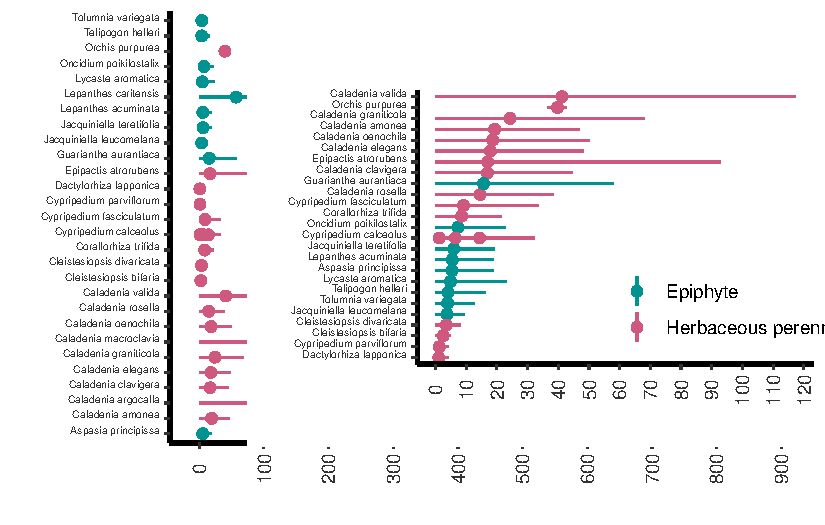
\includegraphics{121-Rage_Largo_y_Expectativa_de_Vida_files/figure-pdf/LV29-1.pdf}

USING Quartiles

\begin{Shaded}
\begin{Highlighting}[]
\NormalTok{longevity\_O }\OtherTok{\textless{}{-}}\NormalTok{ index\_O\_filtrado\_final }\SpecialCharTok{\%\textgreater{}\%}
  \FunctionTok{mutate}\NormalTok{(}
    \AttributeTok{longevidad1 =} \FunctionTok{mapply}\NormalTok{(longevity, matU, }\AttributeTok{start =} \DecValTok{1}\NormalTok{, }\AttributeTok{lx\_crit =} \FloatTok{0.05}\NormalTok{),}
    \AttributeTok{longevidad2 =} \FunctionTok{mapply}\NormalTok{(longevity, matU, }\AttributeTok{start =} \DecValTok{2}\NormalTok{, }\AttributeTok{lx\_crit =} \FloatTok{0.05}\NormalTok{)}
\NormalTok{  ) }\SpecialCharTok{\%\textgreater{}\%}
  \FunctionTok{mutate}\NormalTok{(}\AttributeTok{OrganismType\_RC =} \FunctionTok{fct\_recode}\NormalTok{(OrganismType,}
                                      \StringTok{"Epífita"} \OtherTok{=} \StringTok{"Epiphyte"}\NormalTok{,}
                                      \StringTok{"Terrestre"} \OtherTok{=} \StringTok{"Herbaceous perennial"}\NormalTok{)) }\SpecialCharTok{\%\textgreater{}\%}
  \FunctionTok{group\_by}\NormalTok{(OrganismType\_RC) }\SpecialCharTok{\%\textgreater{}\%}
  \FunctionTok{mutate}\NormalTok{(}
    \AttributeTok{Q1\_longevidad1 =} \FunctionTok{quantile}\NormalTok{(longevidad1, }\FloatTok{0.25}\NormalTok{, }\AttributeTok{na.rm =} \ConstantTok{TRUE}\NormalTok{),}
    \AttributeTok{Q3\_longevidad1 =} \FunctionTok{quantile}\NormalTok{(longevidad1, }\FloatTok{0.75}\NormalTok{, }\AttributeTok{na.rm =} \ConstantTok{TRUE}\NormalTok{),}
    \AttributeTok{median\_longevidad1 =} \FunctionTok{quantile}\NormalTok{(longevidad1, }\FloatTok{0.5}\NormalTok{, }\AttributeTok{na.rm =} \ConstantTok{TRUE}\NormalTok{),}
    \AttributeTok{mean\_longevidad1 =} \FunctionTok{mean}\NormalTok{(longevidad1, }\AttributeTok{na.rm =} \ConstantTok{TRUE}\NormalTok{)}
\NormalTok{  ) }\SpecialCharTok{\%\textgreater{}\%}
  \FunctionTok{ungroup}\NormalTok{()}

\NormalTok{longevity\_O}\SpecialCharTok{$}\NormalTok{SpeciesAccepted }\OtherTok{\textless{}{-}} \FunctionTok{fct\_reorder}\NormalTok{(}
\NormalTok{  longevity\_O}\SpecialCharTok{$}\NormalTok{SpeciesAccepted,}
\NormalTok{  longevity\_O}\SpecialCharTok{$}\NormalTok{mean\_longevidad1,}
  \AttributeTok{.desc =} \ConstantTok{FALSE}
\NormalTok{)}

\NormalTok{main.plot }\OtherTok{\textless{}{-}} \FunctionTok{ggplot}\NormalTok{(longevity\_O, }\FunctionTok{aes}\NormalTok{(}\AttributeTok{x =}\NormalTok{ SpeciesAccepted, }\AttributeTok{color =}\NormalTok{ OrganismType\_RC)) }\SpecialCharTok{+}
  \FunctionTok{geom\_linerange}\NormalTok{(}\FunctionTok{aes}\NormalTok{(}\AttributeTok{ymin =}\NormalTok{ Q1\_longevidad1, }\AttributeTok{ymax =}\NormalTok{ Q3\_longevidad1)) }\SpecialCharTok{+}
  \FunctionTok{geom\_point}\NormalTok{(}\FunctionTok{aes}\NormalTok{(}\AttributeTok{y =}\NormalTok{ longevidad1), }\AttributeTok{size =} \DecValTok{2}\NormalTok{) }\SpecialCharTok{+}
  \FunctionTok{coord\_flip}\NormalTok{() }\SpecialCharTok{+}
  \FunctionTok{theme}\NormalTok{(}\AttributeTok{legend.position.inside =} \FunctionTok{c}\NormalTok{(}\FloatTok{0.8}\NormalTok{, }\FloatTok{0.2}\NormalTok{))}

\NormalTok{main.plot}
\end{Highlighting}
\end{Shaded}

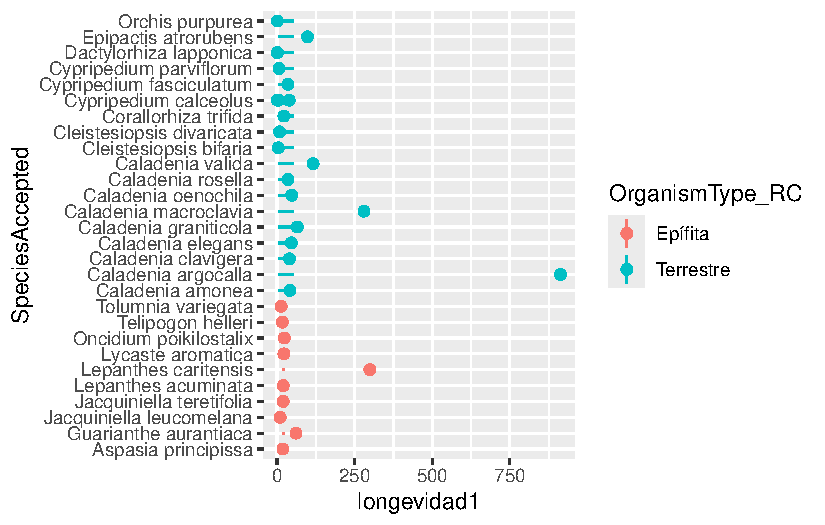
\includegraphics{121-Rage_Largo_y_Expectativa_de_Vida_files/figure-pdf/LV30-1.pdf}

\begin{Shaded}
\begin{Highlighting}[]
\NormalTok{index\_O\_calculado\_median }\OtherTok{\textless{}{-}}\NormalTok{ index\_O\_filtrado\_final }\SpecialCharTok{\%\textgreater{}\%}
  \FunctionTok{mutate}\NormalTok{(}\AttributeTok{life\_expectancy =} \FunctionTok{mapply}\NormalTok{(lifeExpectancy, matU, start\_life)) }\SpecialCharTok{\%\textgreater{}\%}
  \FunctionTok{mutate}\NormalTok{(}\AttributeTok{var\_life\_expectancy =} \FunctionTok{mapply}\NormalTok{(life\_expect\_var, matU, }\AttributeTok{start =} \DecValTok{1}\NormalTok{)) }\SpecialCharTok{\%\textgreater{}\%}
  \FunctionTok{group\_by}\NormalTok{(OrganismType) }\SpecialCharTok{\%\textgreater{}\%}
  \FunctionTok{mutate}\NormalTok{(}
    \AttributeTok{Q1\_life\_expectancy =} \FunctionTok{quantile}\NormalTok{(life\_expectancy, }\FloatTok{0.25}\NormalTok{, }\AttributeTok{na.rm =} \ConstantTok{TRUE}\NormalTok{),}
    \AttributeTok{Median\_life\_expectancy =} \FunctionTok{quantile}\NormalTok{(life\_expectancy, }\FloatTok{0.5}\NormalTok{, }\AttributeTok{na.rm =} \ConstantTok{TRUE}\NormalTok{),}
    \AttributeTok{Q3\_life\_expectancy =} \FunctionTok{quantile}\NormalTok{(life\_expectancy, }\FloatTok{0.75}\NormalTok{, }\AttributeTok{na.rm =} \ConstantTok{TRUE}\NormalTok{)}
\NormalTok{  ) }\SpecialCharTok{\%\textgreater{}\%}
  \FunctionTok{ungroup}\NormalTok{() }\SpecialCharTok{\%\textgreater{}\%}
  \FunctionTok{mutate}\NormalTok{(}\AttributeTok{OrganismType =} \FunctionTok{reorder}\NormalTok{(OrganismType, life\_expectancy, median))}

\NormalTok{index\_O\_calculado\_subset2}\OtherTok{=}\NormalTok{index\_O\_calculado\_median }\SpecialCharTok{|\textgreater{}} 
  \FunctionTok{select}\NormalTok{(mat, SpeciesAccepted, OrganismType, life\_expectancy, Q1\_life\_expectancy, }
\NormalTok{         Q3\_life\_expectancy, Median\_life\_expectancy) }\SpecialCharTok{|\textgreater{}} 
  \FunctionTok{mutate}\NormalTok{(}\AttributeTok{OrganismType\_RC=}\FunctionTok{fct\_recode}\NormalTok{(OrganismType,}
                             \StringTok{"Epífita"}\OtherTok{=}\StringTok{"Epiphyte"}\NormalTok{,}
                             \StringTok{"Terrestre"}\OtherTok{=}\StringTok{"Herbaceous perennial"}\NormalTok{))}


\NormalTok{index\_O\_calculado\_subset2}\SpecialCharTok{$}\NormalTok{SpeciesAccepted }\OtherTok{\textless{}{-}} \FunctionTok{fct\_reorder}\NormalTok{(}
\NormalTok{  index\_O\_calculado\_subset2}\SpecialCharTok{$}\NormalTok{SpeciesAccepted,}
\NormalTok{  index\_O\_calculado\_subset2}\SpecialCharTok{$}\NormalTok{Median\_life\_expectancy,}
  \AttributeTok{.desc =} \ConstantTok{FALSE}
\NormalTok{)}


\NormalTok{main.plot\_median }\OtherTok{\textless{}{-}} \FunctionTok{ggplot}\NormalTok{(index\_O\_calculado\_subset2, }\FunctionTok{aes}\NormalTok{(SpeciesAccepted, }\AttributeTok{color =}\NormalTok{ OrganismType\_RC)) }\SpecialCharTok{+}
  \FunctionTok{geom\_linerange}\NormalTok{(}\FunctionTok{aes}\NormalTok{(}\AttributeTok{x =}\NormalTok{ SpeciesAccepted, }\AttributeTok{ymin =}\NormalTok{ Q1\_life\_expectancy, }\AttributeTok{ymax =}\NormalTok{ Q3\_life\_expectancy)) }\SpecialCharTok{+}
  \FunctionTok{geom\_point}\NormalTok{(}\FunctionTok{aes}\NormalTok{(}\AttributeTok{y =}\NormalTok{ Median\_life\_expectancy), }\AttributeTok{size =} \DecValTok{2}\NormalTok{) }\SpecialCharTok{+}
  \FunctionTok{coord\_flip}\NormalTok{() }\SpecialCharTok{+}
  \FunctionTok{theme}\NormalTok{(}\AttributeTok{legend.position.inside =} \FunctionTok{c}\NormalTok{(}\FloatTok{0.8}\NormalTok{, }\FloatTok{0.2}\NormalTok{))}



\NormalTok{main.plot\_median}
\end{Highlighting}
\end{Shaded}

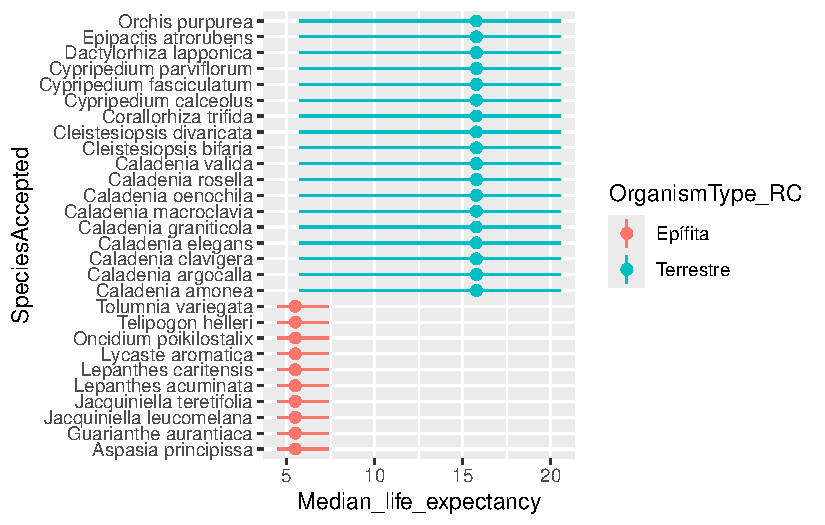
\includegraphics{121-Rage_Largo_y_Expectativa_de_Vida_files/figure-pdf/LV31-1.pdf}

\begin{center}\rule{0.5\linewidth}{0.5pt}\end{center}

\section{Longevidad sin los intervalos de
confianza}\label{longevidad-sin-los-intervalos-de-confianza-1}

La longevidad es el largo de vida máximo que puede alcanzar un individuo
en una población. En este caso se usa la función \textbf{longevity} para
calcular el tiempo para un cohorte llegue a un 5\% de supervivencia. La
función \textbf{longevity} requiere la matriz de transición
\textbf{matU} y la etapa de inicio de la vida \textbf{start\_life}.

\begin{Shaded}
\begin{Highlighting}[]
\CommentTok{\# names(index\_O\_calculado)}

\NormalTok{index\_O\_calculado\_subset}\OtherTok{=}\NormalTok{index\_O\_calculado }\SpecialCharTok{|\textgreater{}} 
  \FunctionTok{select}\NormalTok{(mat, SpeciesAccepted, OrganismType, life\_expectancy, var\_life\_expectancy, }
\NormalTok{         low\_CI\_var\_LS, high\_CI\_var\_LS, OrganismType) }\SpecialCharTok{|\textgreater{}} 
  \FunctionTok{mutate}\NormalTok{(}\AttributeTok{OrganismType\_RC=}\FunctionTok{fct\_recode}\NormalTok{(OrganismType,}
                             \StringTok{"Epífita"}\OtherTok{=}\StringTok{"Epiphyte"}\NormalTok{,}
                             \StringTok{"Terrestre"}\OtherTok{=}\StringTok{"Herbaceous perennial"}\NormalTok{))}


\NormalTok{longevity\_O }\OtherTok{\textless{}{-}}\NormalTok{ index\_O\_filtrado\_final }\SpecialCharTok{\%\textgreater{}\%}
  \FunctionTok{mutate}\NormalTok{(}\AttributeTok{longevidad1=}\FunctionTok{mapply}\NormalTok{(longevity, matU, }\AttributeTok{start =} \DecValTok{1}\NormalTok{, }\AttributeTok{lx\_crit =} \FloatTok{0.05}\NormalTok{),}
         \AttributeTok{longevidad2=}\FunctionTok{mapply}\NormalTok{(longevity, matU, }\AttributeTok{start =} \DecValTok{2}\NormalTok{, }\AttributeTok{lx\_crit =} \FloatTok{0.05}\NormalTok{)) }\CommentTok{\# calcular la longevidad por cada especie}
\end{Highlighting}
\end{Shaded}

\begin{Shaded}
\begin{Highlighting}[]
\CommentTok{\#names(longevity\_O)}

\NormalTok{index\_O\_filtrado\_final }\OtherTok{\textless{}{-}}\NormalTok{ index\_O\_filtrado }\SpecialCharTok{\%\textgreater{}\%}
  \FunctionTok{filter}\NormalTok{(}\FunctionTok{sapply}\NormalTok{(matU, }\ControlFlowTok{function}\NormalTok{(mat) \{}
    \ControlFlowTok{if}\NormalTok{ (}\FunctionTok{is.null}\NormalTok{(mat)) }\FunctionTok{return}\NormalTok{(}\ConstantTok{FALSE}\NormalTok{)}
    \FunctionTok{all}\NormalTok{(}\FunctionTok{colSums}\NormalTok{(mat, }\AttributeTok{na.rm =} \ConstantTok{TRUE}\NormalTok{) }\SpecialCharTok{\textless{}=} \DecValTok{1}\NormalTok{)}
\NormalTok{  \}))}


\NormalTok{longevity\_O }\OtherTok{\textless{}{-}}\NormalTok{ index\_O\_filtrado\_final }\SpecialCharTok{\%\textgreater{}\%}
  \FunctionTok{mutate}\NormalTok{(}\AttributeTok{longevidad1=}\FunctionTok{mapply}\NormalTok{(longevity, matU, }\AttributeTok{start =} \DecValTok{1}\NormalTok{, }\AttributeTok{lx\_crit =} \FloatTok{0.05}\NormalTok{),}
         \AttributeTok{longevidad2=}\FunctionTok{mapply}\NormalTok{(longevity, matU, }\AttributeTok{start =} \DecValTok{2}\NormalTok{, }\AttributeTok{lx\_crit =} \FloatTok{0.05}\NormalTok{)) }\CommentTok{\# calcular la longevidad por cada especie}


\NormalTok{longevity\_O}\OtherTok{=}\NormalTok{longevity\_O}\SpecialCharTok{|\textgreater{}}
\FunctionTok{mutate}\NormalTok{(}\AttributeTok{OrganismType\_RC=}\FunctionTok{fct\_recode}\NormalTok{(OrganismType,}
                            \StringTok{"Epífita"}\OtherTok{=}\StringTok{"Epiphyte"}\NormalTok{,}
                            \StringTok{"Terrestre"}\OtherTok{=}\StringTok{"Herbaceous perennial"}\NormalTok{))}

\NormalTok{longevity\_O}\SpecialCharTok{$}\NormalTok{SpeciesAccepted }\OtherTok{\textless{}{-}} \FunctionTok{fct\_reorder}\NormalTok{(}
\NormalTok{  longevity\_O}\SpecialCharTok{$}\NormalTok{SpeciesAccepted,}
\NormalTok{  longevity\_O}\SpecialCharTok{$}\NormalTok{longevidad1,}
  \AttributeTok{.desc =} \ConstantTok{FALSE}
\NormalTok{)}

\NormalTok{main.plot}\OtherTok{=}\FunctionTok{ggplot}\NormalTok{(longevity\_O , }\FunctionTok{aes}\NormalTok{(}\AttributeTok{x=}\NormalTok{SpeciesAccepted, }\AttributeTok{y=}\NormalTok{longevidad2, }\AttributeTok{color =}\NormalTok{ OrganismType\_RC)) }\SpecialCharTok{+}
  \FunctionTok{geom\_point}\NormalTok{() }\SpecialCharTok{+}
 \FunctionTok{coord\_flip}\NormalTok{() }\SpecialCharTok{+}
  \FunctionTok{theme}\NormalTok{(}\AttributeTok{legend.position.inside =} \FunctionTok{c}\NormalTok{(}\FloatTok{0.8}\NormalTok{, }\FloatTok{0.2}\NormalTok{)) }\SpecialCharTok{+}
  \FunctionTok{ylab}\NormalTok{(}\StringTok{""}\NormalTok{) }\SpecialCharTok{+}
  \FunctionTok{xlab}\NormalTok{(}\StringTok{""}\NormalTok{) }\SpecialCharTok{+}
  \FunctionTok{rlt\_style\_colour}\NormalTok{() }\SpecialCharTok{+}
  \FunctionTok{theme}\NormalTok{(}
    \AttributeTok{axis.text.x =} \FunctionTok{element\_text}\NormalTok{(}
      \AttributeTok{color =} \StringTok{"grey20"}\NormalTok{,}
      \AttributeTok{size =} \DecValTok{9}\NormalTok{,}
      \AttributeTok{angle =} \DecValTok{90}\NormalTok{,}
      \AttributeTok{hjust =}\NormalTok{ .}\DecValTok{5}\NormalTok{,}
      \AttributeTok{vjust =}\NormalTok{ .}\DecValTok{5}\NormalTok{,}
      \AttributeTok{face =} \StringTok{"plain"}
\NormalTok{    ),}
    \AttributeTok{axis.text.y =} \FunctionTok{element\_text}\NormalTok{(}
      \AttributeTok{color =} \StringTok{"grey20"}\NormalTok{,}
      \AttributeTok{size =} \DecValTok{7}\NormalTok{,}
      \AttributeTok{angle =} \DecValTok{0}\NormalTok{,}
      \AttributeTok{hjust =} \DecValTok{1}\NormalTok{,}
      \AttributeTok{vjust =} \DecValTok{0}\NormalTok{,}
      \AttributeTok{face =} \StringTok{"plain"}
\NormalTok{    ),}
    \AttributeTok{axis.title.x =} \FunctionTok{element\_text}\NormalTok{(}
      \AttributeTok{color =} \StringTok{"grey20"}\NormalTok{,}
      \AttributeTok{size =} \DecValTok{12}\NormalTok{,}
      \AttributeTok{angle =} \DecValTok{0}\NormalTok{,}
      \AttributeTok{hjust =}\NormalTok{ .}\DecValTok{5}\NormalTok{,}
      \AttributeTok{vjust =} \DecValTok{0}\NormalTok{,}
      \AttributeTok{face =} \StringTok{"plain"}
\NormalTok{    ),}
    \AttributeTok{axis.title.y =} \FunctionTok{element\_text}\NormalTok{(}
      \AttributeTok{color =} \StringTok{"grey20"}\NormalTok{,}
      \AttributeTok{size =} \DecValTok{12}\NormalTok{,}
      \AttributeTok{angle =} \DecValTok{90}\NormalTok{,}
      \AttributeTok{hjust =}\NormalTok{ .}\DecValTok{5}\NormalTok{,}
      \AttributeTok{vjust =}\NormalTok{ .}\DecValTok{5}\NormalTok{,}
      \AttributeTok{face =} \StringTok{"plain"}
\NormalTok{    )}
\NormalTok{  )}\SpecialCharTok{+}
  \FunctionTok{theme}\NormalTok{(}\AttributeTok{legend.position=}\StringTok{"none"}\NormalTok{)}\SpecialCharTok{+}
  \FunctionTok{theme}\NormalTok{(}\AttributeTok{axis.text.y =} \FunctionTok{element\_text}\NormalTok{(}\AttributeTok{size =} \DecValTok{5}\NormalTok{))}\SpecialCharTok{+}
  \FunctionTok{scale\_y\_continuous}\NormalTok{(}\AttributeTok{n.breaks =} \DecValTok{12}\NormalTok{)}

\DocumentationTok{\#\# Insertar la figura con las especies con longevidad \textless{}50 años}

\NormalTok{inset.plot}\OtherTok{=}\NormalTok{longevity\_O }\SpecialCharTok{|\textgreater{}} 
  \FunctionTok{filter}\NormalTok{(longevidad2 }\SpecialCharTok{\textless{}}\DecValTok{50}\NormalTok{) }\SpecialCharTok{|\textgreater{}} 
\FunctionTok{ggplot}\NormalTok{(}\FunctionTok{aes}\NormalTok{(}\AttributeTok{x=}\NormalTok{SpeciesAccepted, }\AttributeTok{y=}\NormalTok{longevidad2, }\AttributeTok{color =}\NormalTok{ OrganismType\_RC)) }\SpecialCharTok{+}
  \FunctionTok{geom\_point}\NormalTok{() }\SpecialCharTok{+}
  \FunctionTok{coord\_flip}\NormalTok{() }\SpecialCharTok{+}
  \FunctionTok{theme}\NormalTok{(}\AttributeTok{legend.position.inside =} \FunctionTok{c}\NormalTok{(}\FloatTok{0.8}\NormalTok{, }\FloatTok{0.2}\NormalTok{)) }\SpecialCharTok{+}
  \FunctionTok{ylab}\NormalTok{(}\StringTok{""}\NormalTok{) }\SpecialCharTok{+}
  \FunctionTok{xlab}\NormalTok{(}\StringTok{""}\NormalTok{) }\SpecialCharTok{+}
  \FunctionTok{rlt\_style\_colour}\NormalTok{() }\SpecialCharTok{+}
  \FunctionTok{theme}\NormalTok{(}
    \AttributeTok{axis.text.x =} \FunctionTok{element\_text}\NormalTok{(}
      \AttributeTok{color =} \StringTok{"grey20"}\NormalTok{,}
      \AttributeTok{size =} \DecValTok{9}\NormalTok{,}
      \AttributeTok{angle =} \DecValTok{90}\NormalTok{,}
      \AttributeTok{hjust =}\NormalTok{ .}\DecValTok{5}\NormalTok{,}
      \AttributeTok{vjust =}\NormalTok{ .}\DecValTok{5}\NormalTok{,}
      \AttributeTok{face =} \StringTok{"plain"}
\NormalTok{    ),}
    \AttributeTok{axis.text.y =} \FunctionTok{element\_text}\NormalTok{(}
      \AttributeTok{color =} \StringTok{"grey20"}\NormalTok{,}
      \AttributeTok{size =} \DecValTok{7}\NormalTok{,}
      \AttributeTok{angle =} \DecValTok{0}\NormalTok{,}
      \AttributeTok{hjust =} \DecValTok{1}\NormalTok{,}
      \AttributeTok{vjust =} \DecValTok{0}\NormalTok{,}
      \AttributeTok{face =} \StringTok{"plain"}
\NormalTok{    ),}
    \AttributeTok{axis.title.x =} \FunctionTok{element\_text}\NormalTok{(}
      \AttributeTok{color =} \StringTok{"grey20"}\NormalTok{,}
      \AttributeTok{size =} \DecValTok{12}\NormalTok{,}
      \AttributeTok{angle =} \DecValTok{0}\NormalTok{,}
      \AttributeTok{hjust =}\NormalTok{ .}\DecValTok{5}\NormalTok{,}
      \AttributeTok{vjust =} \DecValTok{0}\NormalTok{,}
      \AttributeTok{face =} \StringTok{"plain"}
\NormalTok{    ),}
    \AttributeTok{axis.title.y =} \FunctionTok{element\_text}\NormalTok{(}
      \AttributeTok{color =} \StringTok{"grey20"}\NormalTok{,}
      \AttributeTok{size =} \DecValTok{12}\NormalTok{,}
      \AttributeTok{angle =} \DecValTok{90}\NormalTok{,}
      \AttributeTok{hjust =}\NormalTok{ .}\DecValTok{5}\NormalTok{,}
      \AttributeTok{vjust =}\NormalTok{ .}\DecValTok{5}\NormalTok{,}
      \AttributeTok{face =} \StringTok{"plain"}
\NormalTok{    )}
\NormalTok{  )}\SpecialCharTok{+}
  \FunctionTok{theme}\NormalTok{(}\AttributeTok{legend.position =} \FunctionTok{c}\NormalTok{(}\FloatTok{0.8}\NormalTok{,}\FloatTok{0.2}\NormalTok{),}
        \AttributeTok{legend.title =} \FunctionTok{element\_blank}\NormalTok{())}\SpecialCharTok{+}
  \FunctionTok{theme}\NormalTok{(}\AttributeTok{axis.text.y =} \FunctionTok{element\_text}\NormalTok{(}\AttributeTok{size =} \DecValTok{5}\NormalTok{))}\SpecialCharTok{+}
  \FunctionTok{scale\_y\_continuous}\NormalTok{(}\AttributeTok{n.breaks =} \DecValTok{12}\NormalTok{)}

\FunctionTok{library}\NormalTok{(cowplot)}

\NormalTok{longevidad\_plot }\OtherTok{\textless{}{-}} \FunctionTok{ggdraw}\NormalTok{() }\SpecialCharTok{+}
  \FunctionTok{draw\_plot}\NormalTok{(main.plot) }\SpecialCharTok{+}
  \FunctionTok{draw\_plot}\NormalTok{(inset.plot, }\AttributeTok{x =} \FloatTok{0.3}\NormalTok{, }\AttributeTok{y =} \FloatTok{0.15}\NormalTok{, }\AttributeTok{width =} \FloatTok{0.7}\NormalTok{, }\AttributeTok{height =} \FloatTok{0.7}\NormalTok{)}

\NormalTok{longevidad\_plot}
\end{Highlighting}
\end{Shaded}

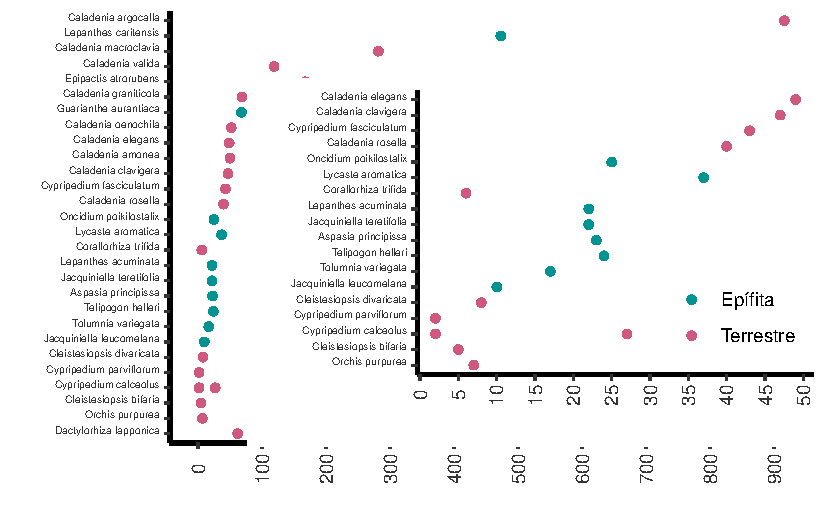
\includegraphics{121-Rage_Largo_y_Expectativa_de_Vida_files/figure-pdf/LV33-1.pdf}

\subsubsection{}\label{section-1}

Estimar el largo de

Figura del largo de vida promedio y su varianza para las orquídeas
terrestres y epifitas.

\begin{Shaded}
\begin{Highlighting}[]
\NormalTok{lifeExpectancy }\OtherTok{\textless{}{-}} \ControlFlowTok{function}\NormalTok{(matU, startLife) \{}
\NormalTok{  N }\OtherTok{\textless{}{-}} \FunctionTok{solve}\NormalTok{(}\FunctionTok{diag}\NormalTok{(}\FunctionTok{nrow}\NormalTok{(matU)) }\SpecialCharTok{{-}}\NormalTok{ matU)}
  \FunctionTok{return}\NormalTok{(}\FunctionTok{colSums}\NormalTok{(N)[startLife])}
\NormalTok{\}}


\NormalTok{compadre\_life\_expect }\OtherTok{\textless{}{-}}\NormalTok{ Orquideas }\SpecialCharTok{\%\textgreater{}\%}
  \FunctionTok{filter}\NormalTok{(ProjectionInterval }\SpecialCharTok{==} \FloatTok{1.0}\NormalTok{) }\SpecialCharTok{|\textgreater{}} \CommentTok{\# filtrar para matriz de un año solamente}
  \FunctionTok{filter}\NormalTok{(}
\NormalTok{    MatrixComposite }\SpecialCharTok{==} \StringTok{"Mean"}\NormalTok{, }\CommentTok{\# filtrar para la matriz promedia}
\NormalTok{    MatrixTreatment }\SpecialCharTok{==} \StringTok{"Unmanipulated"}\NormalTok{, }\CommentTok{\# filtrar para la matriz sin manipulación}
\NormalTok{    MatrixCaptivity }\SpecialCharTok{==} \StringTok{"W"} \CommentTok{\# filtrar para poblaciones naturales (no en cautiverio)}
\NormalTok{  ) }\SpecialCharTok{\%\textgreater{}\%}
  \FunctionTok{mutate}\NormalTok{(}\AttributeTok{StageID =} \FunctionTok{cdb\_id\_stages}\NormalTok{(.)) }\SpecialCharTok{\%\textgreater{}\%} \CommentTok{\# crear un ID para las etapas}
  \FunctionTok{cdb\_collapse}\NormalTok{(}\AttributeTok{columns =} \StringTok{"StageID"}\NormalTok{) }\SpecialCharTok{\%\textgreater{}\%} \CommentTok{\# colapsar las etapas}
  \FunctionTok{cdb\_flag}\NormalTok{() }\SpecialCharTok{\%\textgreater{}\%} \CommentTok{\# evaluar las matrices y crear una columna para cada evaluación}
  \FunctionTok{filter}\NormalTok{(}
\NormalTok{    check\_NA\_U }\SpecialCharTok{==} \ConstantTok{FALSE}\NormalTok{, }\CommentTok{\# filtrar para matrices sin valores faltantes}
\NormalTok{    check\_zero\_U }\SpecialCharTok{==} \ConstantTok{FALSE}\NormalTok{, }\CommentTok{\# filtrar para matrices sin valores cero}
\NormalTok{    check\_singular\_U }\SpecialCharTok{==} \ConstantTok{FALSE}\NormalTok{,}
\NormalTok{    check\_surv\_gte\_1 }\SpecialCharTok{==} \ConstantTok{FALSE}\NormalTok{, }\CommentTok{\# filtrar para matrices sin valores de supervivencia mayores a 1}
\NormalTok{  ) }\SpecialCharTok{\%\textgreater{}\%} \CommentTok{\# filtrar para matrices no singulares}
  \FunctionTok{mutate}\NormalTok{(}\AttributeTok{matU =} \FunctionTok{matU}\NormalTok{(.), }\AttributeTok{start\_life =} \FunctionTok{mpm\_first\_active}\NormalTok{(.)) }\SpecialCharTok{\%\textgreater{}\%} \CommentTok{\# extraer la matriz de transición y la etapa de inicio de la vida}
  \FunctionTok{mutate}\NormalTok{(}\AttributeTok{life\_expectancy =} \FunctionTok{mapply}\NormalTok{(lifeExpectancy, matU, start\_life)) }\SpecialCharTok{\%\textgreater{}\%} \CommentTok{\# calcular el largo de vida}
  \FunctionTok{mutate}\NormalTok{(}\AttributeTok{var\_life\_expectancy =} \FunctionTok{mapply}\NormalTok{(life\_expect\_var, matU, }\AttributeTok{start =} \DecValTok{1}\NormalTok{)) }\SpecialCharTok{\%\textgreater{}\%} \CommentTok{\# calcular la varianza del largo de vida}
  \FunctionTok{mutate}\NormalTok{(}\AttributeTok{low\_CI\_var\_LS =}\NormalTok{ life\_expectancy }\SpecialCharTok{{-}} \FloatTok{1.96} \SpecialCharTok{*} \FunctionTok{sqrt}\NormalTok{(var\_life\_expectancy)) }\SpecialCharTok{\%\textgreater{}\%} \CommentTok{\# calcular el intervalo de confianza inferior}
  \FunctionTok{mutate}\NormalTok{(}
    \AttributeTok{high\_CI\_var\_LS =}\NormalTok{ life\_expectancy }\SpecialCharTok{+} \FloatTok{1.96} \SpecialCharTok{*} \FunctionTok{sqrt}\NormalTok{(var\_life\_expectancy)) }\SpecialCharTok{\%\textgreater{}\%} \CommentTok{\# calcular el intervalo de confianza superior}
  \FunctionTok{mutate}\NormalTok{(}\AttributeTok{OrganismType =} \FunctionTok{reorder}\NormalTok{(OrganismType, life\_expectancy, median)) }\CommentTok{\# ordenar las especies por el largo de vida}
\end{Highlighting}
\end{Shaded}

Visualizar el largo de vida por plantas epifitas versus terrestres. Nota
aquí que algunas especies están representada múltiple veces. Por
consecuencia la distribución de los datos no es una buena representación
de la diferencia entre las especies epifitas y terrestres, debido a lo
que se llama pseudoreplicación. Este tabla representa la distribución
los datos del data frame anterior.

Calculando el promedio y la desviación estándar de la esperanza de vida
de las orquídeas.

\begin{Shaded}
\begin{Highlighting}[]
\NormalTok{index\_O\_calculado }\SpecialCharTok{|\textgreater{}}
  \FunctionTok{group\_by}\NormalTok{(OrganismType) }\SpecialCharTok{|\textgreater{}}
  \FunctionTok{summarize}\NormalTok{(}
    \AttributeTok{mean\_LS =} \FunctionTok{mean}\NormalTok{(life\_expectancy, }\AttributeTok{na.rm =} \ConstantTok{TRUE}\NormalTok{),}
    \AttributeTok{sd\_LS =} \FunctionTok{sd}\NormalTok{(var\_life\_expectancy, }\AttributeTok{na.rm =} \ConstantTok{TRUE}\NormalTok{)}
\NormalTok{  )}


\CommentTok{\#OrchidLS |\textgreater{}}
\CommentTok{\#  group\_by(OrganismType) |\textgreater{}}
\CommentTok{\#  summarize(}
 \CommentTok{\#   mean\_LS = mean(life\_expectancy, na.rm = TRUE),}
 \CommentTok{\#   sd\_LS = sd(life\_expectancy, na.rm = TRUE)}
\CommentTok{\#  )}
\end{Highlighting}
\end{Shaded}

Haciendo una figura del largo de vida de las especies epífitas y
terrestres. Nota que la escala es logarítmica.

\begin{Shaded}
\begin{Highlighting}[]
\NormalTok{ggplot2}\SpecialCharTok{::}\FunctionTok{ggplot}\NormalTok{(}
\NormalTok{  index\_O\_calculado,}
  \FunctionTok{aes}\NormalTok{(OrganismType, life\_expectancy, }\AttributeTok{colour =}\NormalTok{ OrganismType)}
\NormalTok{) }\SpecialCharTok{+}
  \FunctionTok{geom\_boxplot}\NormalTok{(}\AttributeTok{size=}\NormalTok{.}\DecValTok{8}\NormalTok{) }\SpecialCharTok{+}
  \FunctionTok{geom\_point}\NormalTok{() }\SpecialCharTok{+}
  \FunctionTok{scale\_y\_log10}\NormalTok{() }\SpecialCharTok{+}
  \FunctionTok{coord\_flip}\NormalTok{() }\SpecialCharTok{+}
  \FunctionTok{labs}\NormalTok{(}\AttributeTok{x =} \ConstantTok{NULL}\NormalTok{, }\AttributeTok{y =} \StringTok{"Life expectancy (log(years))"}\NormalTok{) }\SpecialCharTok{+}
\NormalTok{  rlt\_theme }\SpecialCharTok{+}
  \FunctionTok{theme}\NormalTok{(}\AttributeTok{legend.position =} \StringTok{"none"}\NormalTok{)}

\FunctionTok{ggsave}\NormalTok{(}\StringTok{"Figures/Life\_Span.png"}\NormalTok{)}
\end{Highlighting}
\end{Shaded}

https://jonesor.github.io/Rage/reference/life\_expect.html

En el siguiente script y gráfico vemos la visualización por genero de
los estimados de la esperanza de vida. Nota que la esperanza de vida es
un estimado y no un valor exacto. En este caso se usa la función
\textbf{life\_expect\_var} para calcular la varianza de la esperanza de
vida. La escala de x (el largo de vida fue cambiado a log10 de la
esperanza de vida).

\textbf{How to calculate CI of life span, it is in the table above, use
gamma, not normal} !!!!

low\_CI\_var\_LS high\_CI\_var\_LS

\begin{Shaded}
\begin{Highlighting}[]
\CommentTok{\#SPECIES\_O$SpeciesAccepted \textless{}{-} fct\_reorder(SPECIES\_O$SpeciesAccepted, SPECIES\_O$StudyStart, .desc = FALSE) \# Ordenar por fecha de inicio del estudio}


\FunctionTok{ggplot}\NormalTok{(}
\NormalTok{  index\_O\_calculado,}
  \FunctionTok{aes}\NormalTok{(}
    \AttributeTok{x =} \FunctionTok{reorder}\NormalTok{(SpeciesAccepted, life\_expectancy),}
\NormalTok{    life\_expectancy,}
    \AttributeTok{colour =}\NormalTok{ OrganismType}
\NormalTok{  )}
\NormalTok{) }\SpecialCharTok{+}
  \CommentTok{\# geom\_boxplot() +}
  \FunctionTok{geom\_point}\NormalTok{() }\SpecialCharTok{+}
  \FunctionTok{scale\_y\_log10}\NormalTok{() }\SpecialCharTok{+}
  \FunctionTok{coord\_flip}\NormalTok{() }\SpecialCharTok{+}
  \FunctionTok{labs}\NormalTok{(}\AttributeTok{x =} \ConstantTok{NULL}\NormalTok{, }\AttributeTok{y =} \StringTok{"Life expectancy (log(years))"}\NormalTok{)}
\CommentTok{\#  rlt\_theme+}
\CommentTok{\#theme(legend.position = "none")}

\CommentTok{\#ggsave("Figures/Genus\_Life\_Span.png")}
\end{Highlighting}
\end{Shaded}

EWl largo de vida de las Caladenia solamente

Evaluando el largo de vida de las especies de \emph{Caladenia} solamente

\begin{Shaded}
\begin{Highlighting}[]
\CommentTok{\#SPECIES\_O$SpeciesAccepted \textless{}{-} fct\_reorder(SPECIES\_O$SpeciesAccepted, SPECIES\_O$StudyStart, .desc = FALSE)}

\NormalTok{index\_O\_calculado }\SpecialCharTok{|\textgreater{}}
  \FunctionTok{group\_by}\NormalTok{(Genus) }\SpecialCharTok{|\textgreater{}}
  \FunctionTok{summarize}\NormalTok{(}
    \AttributeTok{mean\_LS =} \FunctionTok{mean}\NormalTok{(life\_expectancy, }\AttributeTok{na.rm =} \ConstantTok{TRUE}\NormalTok{),}
    \AttributeTok{sd\_LS =} \FunctionTok{sd}\NormalTok{(life\_expectancy, }\AttributeTok{na.rm =} \ConstantTok{TRUE}\NormalTok{)}
\NormalTok{  ) }\SpecialCharTok{|\textgreater{}}
  \FunctionTok{filter}\NormalTok{(Genus }\SpecialCharTok{\%in\%} \FunctionTok{c}\NormalTok{(}\StringTok{"Caladenia"}\NormalTok{))}

\NormalTok{index\_O\_calculado }\SpecialCharTok{|\textgreater{}}
  \FunctionTok{filter}\NormalTok{(Genus }\SpecialCharTok{\%in\%} \FunctionTok{c}\NormalTok{(}\StringTok{"Caladenia"}\NormalTok{)) }\SpecialCharTok{|\textgreater{}}
  \FunctionTok{ggplot}\NormalTok{(}\FunctionTok{aes}\NormalTok{(}
    \AttributeTok{x =} \FunctionTok{reorder}\NormalTok{(SpeciesAccepted, life\_expectancy),}
\NormalTok{    life\_expectancy,}
    \AttributeTok{colour =}\NormalTok{ OrganismType}
\NormalTok{  )) }\SpecialCharTok{+}
  \FunctionTok{geom\_point}\NormalTok{() }\SpecialCharTok{+}
  \FunctionTok{scale\_y\_log10}\NormalTok{() }\SpecialCharTok{+}
  \FunctionTok{coord\_flip}\NormalTok{() }\SpecialCharTok{+}
  \FunctionTok{labs}\NormalTok{(}\AttributeTok{x =} \ConstantTok{NULL}\NormalTok{, }\AttributeTok{y =} \StringTok{"Life expectancy (years)"}\NormalTok{) }\SpecialCharTok{+}
\NormalTok{  rlt\_theme }\SpecialCharTok{+}
  \FunctionTok{theme}\NormalTok{(}\AttributeTok{legend.position =} \StringTok{"none"}\NormalTok{)}

\CommentTok{\#ggsave("Figures/Caladenia\_Life\_Span.png")}
\end{Highlighting}
\end{Shaded}

\subsection{Calcular el promedio y la varianza en la expectativa de vida
de un modelo de matriz
poblacional}\label{calcular-el-promedio-y-la-varianza-en-la-expectativa-de-vida-de-un-modelo-de-matriz-poblacional-1}


\backmatter


\end{document}
